\documentclass[a4paper,12pt]{report}
\usepackage{tikz}
\usepackage[hidelinks=true,bookmarksdepth=3]{hyperref}
\usepackage[a4paper,top=2cm, bottom = 2cm, left = 2cm, right = 4cm, marginparsep=-190.2mm]{geometry}
%\usepackage[a4paper,left = 3cm, right = 3cm]{geometry}
\usepackage{amsmath}
\usepackage{mathrsfs}
\usepackage{euscript}
\usepackage[fontsize={14,20}]{xepersian}
\settextfont[Scale=1]{B Nazanin}
%\setlatintextfont[Scale = 1]{Times New Roman}
\DeclareMathAlphabet{\mathpzc}{OT1}{pzc}{m}{it}
\begin{document}
	\begin{center}
		\thispagestyle{empty}
%		*******************************************************************
		\vspace*{1cm}
		\begin{figure}
			\begin{center}
				
\includegraphics[width=4cm, height=4cm]{UniversityLogo}
			\end{center}
		\end{figure}
%		*******************************************************************
		\vspace{-1cm}
		\Large{
			\textbf{دانشگاه اصفهان \lr{-} پردیس خوانسار \\
				دانشکده ریاضی و کامپیوتر \\
			}
		}
%		*******************************************************************
		\vspace{2cm}
		\LARGE{	
			ترجمه فصل 5 کتاب
			
			 \textbf{\lr{Neural Network Design}}
			 			 
			  ویرایش دوم از
			 \lr{Martin T.Hagan}
		}\\
%		*******************************************************************
		\vspace{2cm}		
		\Large{
			مترجمان:
			\textbf{
			عرفان ریاحی، علی کشوری\\			
			}
			استاد:
			\textbf{
				دکتر علی فتاحی\\
			}
		}
%		*******************************************************************
		\vspace{2cm}		
		\Large{
			نیمسال تحصیلی: \textbf{1399 \lr{-} 1400}\\
			نگارش شده با \textbf{\lr{\LaTeX}}
		}
	\end{center}
	\thispagestyle{empty}
	\textcolor{blue}{\textbf{\Huge{5 }\huge{سیگنال و وزن فضاهای برداری}}}\\
	
		\begin{center}
			\begin{tabular}{r r}
				اهداف \hspace{7cm} & 5-1\\
				
				تئوری و مثال‌ها & 5-1\\
				
				فضاهای برداری خطی & 5-2\\
				
				\hspace{1cm}مستقل خطی & 5-4\\
				
				\hspace{1cm}پدید آوردن یک فضا & 5-5\\
				
				\hspace{1cm}ضرب داخلی & 5-6\\
				
				\hspace{1cm}نُرم & 5-6\\
				
				\hspace{1cm}تعامد & 5-7\\
				
				\hspace{2cm}تعامد گرام-اشمیت & 5-7\\
				 
				\hspace{1cm}بسط بردار & 5-9\\

				\hspace{2cm}بردارهای پایه متقابل & 5-10\\
				
				خلاصه نتایج & 5-13\\
				
				  سخن آخر & 5-24\\ 
				  
				  سخن آخر & 5-25\\
				  
				  تمرینات & 5-26\\				  
			\end{tabular}
		\end{center}
%	خودمحوری گرام اشمیت \hspace{4cm} 5-8\\

	\noindent\textbf{\Large{اهداف}}
	\hrule \vspace{0.3cm}	
			بر اساس فصل های 3 و 4 واضح است که فکر کردن به ورودی ها و خروجی های یک شبکه عصبی و درنظر گرفتن سطرهای یک ماتریس وزن به عنوان بردارها، بسیار مفید است. در این فصل ما می‌خواهیم با امتحان کردن فضاهای برداری به صورت مفصل و بازبینی ویژگی های فضاهای برداری که به هنگام تحلیل شبکه‌های عصبی، بسیار مفید واقع می‌شود. ما با تعاریف کلی شروع خواهیم کرد و سپس این تعاریف را برای مشکلات خاص شبکه عصبی به کار می‌بریم. این مفاهیم که در این فصل و فصل بعدی مورد بحث قرار گرفته اند، به طور گسترده در کل فصل‌های باقیمانده کتاب مورد استفاده قرار خواهند گرفت. آنها برای درک ما از چرایی کار شبکه های عصبی، حیاتی هستند.\\
			
	\noindent\textbf{\Large{تئوری و مثال‌ها}}
	\hrule \vspace{0.3cm}
	جبر خطی، هسته ریاضیات مورد نیاز برای درک شبکه های عصبی است. در فصل 3 و 4، ما کارایی معرفی کردن ورودی‌ها و خروجی‌های یک شبکه‌ی عصبی را به عنوان بردار، دیدیم. به علاوه، دیدم که درنظر گرفتن سطرهای یک ماتریس وزنی به عنوان بردارهای ورودی در یک فضای برداری یکسان اغلب مفید است.
	
	از فصل 3 به یاد داریم که در شبکه همینگ سطرهای ماتریس وزن در لایه اولیه با بردارهای نمونه برابر است. در واقع، هدف از لایه اولیه محاسبه ضرب داخلی بین بردارهای نمونه و بردار ورودی بود.
	
	در شبکه‌ی پرسپترون نرونی تکی، ما متذکر شدیم که مرز تصمیم گیری همیشه بر ماتریس وزنی متعامد است.(یک سطر بردار)
	
	در این فصل ما می‌خواهیم مفاهیم پایه از فضاهای برداری را(به عنوان مثال ضرب داخلی، متعامد) در زمینه شبکه های عصبی بازبینی کنیم. ما با تعریف کلی فضاهای برداری شروع خواهیم کرد. سپس ما ویژگی‌های پایه از بردارها که در برنامه‌های شبکه عصبی بسیار مفید هستند را ارائه خواهیم داد.
	
	نکته‌ای قبل از شروع! همه بردارهایی که تا الان در مورد آنها بحث کرده‌ایم، \lr{n}-تایی(ستون‌هایی) از اعداد حقیقی مرتب شده هستند و ما آنها را با حروف کوچک پررنگ نشان داده ایم، به عنوان مثال:
	
	 $$
	 \textbf{\lr{x}}=[x_1 x_2 ... x_n]^T \hspace{3cm} (5.1)
	 $$
	
	این بردارها در $ \Re^n $، فضای اقلیدسی \lr{n}-بعدی استاندارد هستند. در این فصل ما همچنین در مورد فضاهای برداری، کلی تر از $ \Re^n $ صحبت خواهیم کرد. این بردارهای کلی‌تر با حروف نوشتاری مانند $ x $ نمایش داده می شوند. ما در این فصل نشان خواهیم داد که چگونه این بردارهای کلی را اغلب می توان با ستونی از اعداد نشان داد.\\	
	
	\noindent\textbf{\Large{فضاهای بردار خطی}}
	
	منظور ما از فضای برداری چیست؟ ما با یک تعریف بسیار کلی شروع خواهیم کرد. اگرچه این تعریف انتزاعی به نظر می رسد ، ما مثالهای عینی بسیاری را ارائه خواهیم داد. با استفاده از یک تعریف کلی می توان دسته وسیعی از مشکلات را حل کرد ، و می توان درک عمیق تری از مفاهیم را ارائه داد.\\
	
	\textbf{فضای برداری}: یک فضای بردار خطی ، مجموعه ای از عناصر (بردارها) تعریف شده در یک میدان اسکالر است ، که شرایط زیر را برآورده می کند:
	
	1.	عملیاتی به نام جمع برداری به گونه ای تعریف می شود که اگر
	 $ \mathpzc{x} \in X $ ($ \mathpzc{x} $
	  یک عنصر از \lr{X} است) و
	   $ \mathpzc{y} \in X $،
	    آنگاه 
	    $ \mathpzc{x+y} \in X $.\\
	
	2. $ \mathpzc{x+y=y+x} $\\
	
	3. $ \mathpzc{(x+y)+z=x+(y+z)} $\\
	
	4.	یک بردار منحصر به فرد وجود دارد:
	 $ 0 \in X $
	  که بردار صفر نامیده می‌شود، به طوری که
	 $ \mathpzc{x+0=x} $ 
	   برای همه
	 $ \mathpzc{x} \in X $.\\
	
	5. برای هر بردار 
	$ \mathpzc{x} \in X $
	 یک بردار یکتا در $ X $ وجود دارد که
	$ \mathpzc{-x} $
	 نامیده می‌شود، مانند 
	$ \mathpzc{x+(-x)=0} $.\\
	
	6. عملیاتی به نام ضرب تعریف می‌شود به این صورت که برای همه اسکالرها 
	$ a \in F $
	 و همه‌ی بردارها
	$ \mathpzc{x} \in X $ و $ a\mathpzc{x} \in X $.\\
	
	7. برای هر 
	$ \mathpzc{x} \in X $
	و
	$ 1\mathpzc{x}=\mathpzc{x} $
	 (برای اسکالر 1)\\
	
	8. برای دو اسکالر $ a \in F $ و $ b \in F $ و هر 
	$ \mathpzc{x} \in X $ ، $ a(b\mathpzc{x})=(ab)\mathpzc{x} $.\\
	
	9. $ (a+b)\mathpzc{x}=a\mathpzc{x}+b\mathpzc{x} $\\
	
	10. $ a(\mathpzc{x+y}) = a\mathpzc{x}+a\mathpzc{y} $\\
	
	برای نشان دادن این شرایط ، بیایید چند مجموعه نمونه را بررسی کنیم و تعیین کنیم که آیا آنها فضاهای برداری هستند یا نه. 
	\marginpar
	{
		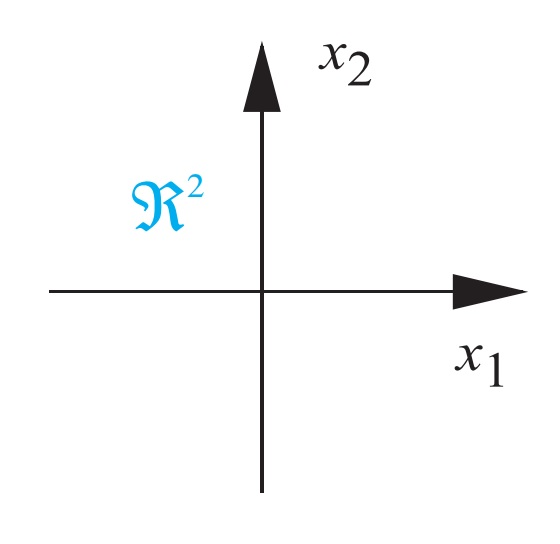
\includegraphics[width=4cm, height=4cm]{124-1}	
	}
	ابتدا فضای اقلیدسی دو بعدی استاندارد را در نظر بگیرید، $ \Re^2 $، که در شکل بالا سمت چپ نشان داده شده است. این به وضوح یک فضای بردار است ، و هر ده شرط برای تعاریف استاندارد جمع بردار و ضرب اسکالر وجود دارد.\\
	
	درمورد زیرمجموعه‌های $ \Re^2 $ چطور؟ کدام زیرمجوعه‌های $ \Re^2 $ نیز فضای برداری هستند؟(زیرفضا) ناحیه مربعی ($ X $) را در شکل سمت راست در نظر بگیرید. آیا همه ده شرط را برآورده می‌کند؟ نه. واضح است که حتی شرط 1 را نیز برآورده نمی‌کند. بردارهای $ \mathpzc{x} $ و $ \mathpzc{y} $ نشان داده شده در شکل در $ X $ قرار دارند، اما بردار $ \mathpzc{x+y} $ اینطور نیست. از این مثال مشخص است که هیچ مجموعه محدودی نمی‌تواند فضای بردار باشد.\\
	\marginpar
	{
		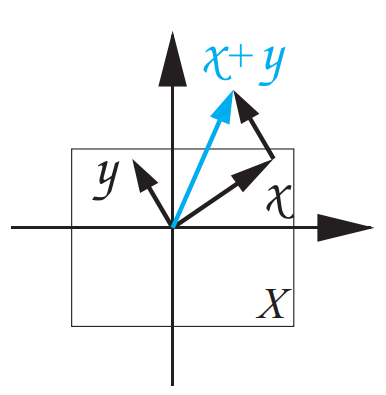
\includegraphics[width=4cm, height=4cm]{124-2}	
	}
	
	آیا زیرمجموعه هایی از $ \Re^2 $ وجود دارد که فضای بردار باشند؟ خط نشان داده در پایین شکل سمت راست را در نظر بگیرید.(فرض کنید که خط از هر دو جهت تا بی نهایت امتداد دارد.) آیا این خط یک فضای بردار است؟ ما این کار را به شما می‌سپاریم تا نشان دهید که در واقع هر ده شرط برآورده شده است. آیا چنین خط نامحدودی ده شرط را برآورده می‌کند؟ خب، هر خطی که از مبدا عبور کند، کارساز خواهد بود. اگر از مبدا عبور نكرد، به عنوان مثال شرط 4 برآورده نمی‌شود.\\
	\marginpar
	{
		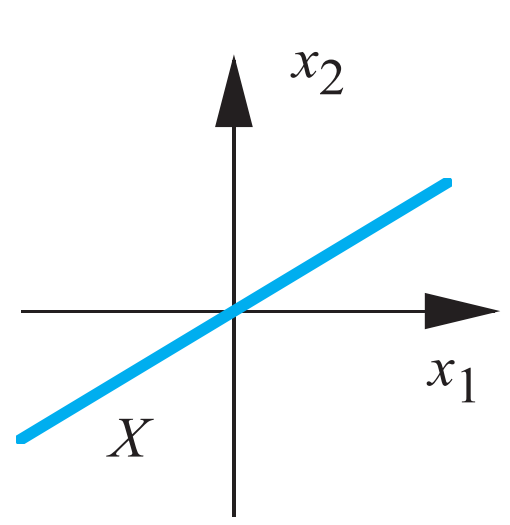
\includegraphics[width=4cm, height=4cm]{124-3}	
	}

	علاوه بر فضاهای استاندارد اقلیدسی، مجموعه های دیگری نیز وجود دارند که ده شرط فضای بردار را نیز برآورده می‌کنند. به عنوان مثال مجموعه $ P^2 $ را تمام چند جمله‌ای‌ها با درجه کمتر یا مساوی 2 در نظر بگیرید. دو   عضو این مجموعه اینها خواهند بود:\\
	$$
	\mathpzc{x}=2+t+4t^2
	$$
	$$
	\hspace{3.5cm} \mathpzc{y}=1+5t \hspace{3cm}  (5.2)
	$$
	
	اگر عادت کرده اید که بردارها را فقط به عنوان ستونی از اعداد در نظر بگیرید، در واقع ممکن است اینها بردارهای عجیبی به نظر برسند. با این حال به یاد بیاورید برای اینکه این یک فضای برداری باشد، یک مجموعه فقط باید ده شرط ارائه شده را برآورده کند. آیا این شرایط برای مجموعه $ P^2 $ راضی کننده است؟ اگر دو چندجمله‌ای با درجه کمتر یا مساوی 2 اضافه کنیم، نتیجه نیز چندجمله‌ای با درجه کمتر یا مساوی 2 خواهد بود. بنابراین شرط 1 برآورده می‌شود. همچنین می‌توانیم یک چندجمله‌ای را در یک اسکالر ضرب کنیم، بدون اینکه ترتیب چندجمله‌ای تغییر کند. بنابراین شرط 6 نیز برآورده می‌شود. نشان دادن اینکه $ P^2 $ یک فضای برداری است، به آسانی اثبات ده شرط گفته شده است.

	مجموعه $ C_{[0,1]} $ را برای تمام توابع پیوسته تعریف شده در بازه $ [0,1] $ در نظر بگیرید. دو عضو این مجموعه موارد زیر خواهند بود:
	$$
	 \mathpzc{x}=sin(t) 
	$$
	$$
	\hspace{3.5cm}  \mathpzc{y}=e^{-2t} \hspace{3cm} (5.3)
	$$ 
	
	یکی دیگر از اعضای مجموعه در شکل سمت چپ نشان داده شده است.
	
	\marginpar
	{
		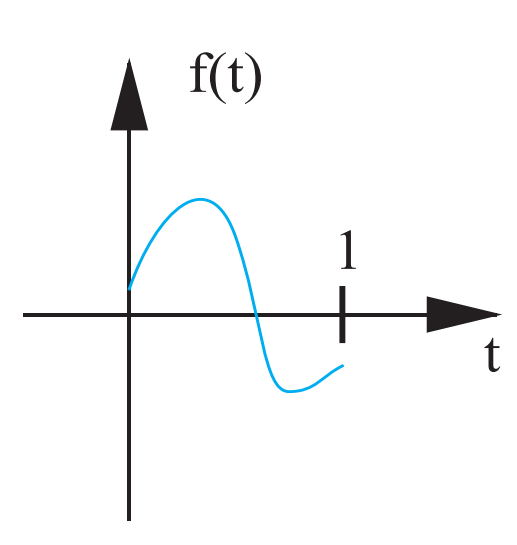
\includegraphics[width=4cm, height=4cm]{125-1}	
	}
	
	مجموع دو تابع پیوسته نیز یک تابع پیوسته است و ضرب اسکالر در یک تابع پیوسته، یک تابع پیوسته است. همچنین مجموعه $ C_{[0,1]} $ یک فضای برداری است. این مجموعه با سایر فضاهای برداری که بحث کردیم متفاوت است. این ابعاد بی‌نهایت است. منظور ما از بُعد را بعداً در این فصل تعریف خواهیم کرد.\\
	
	\noindent\textbf{\Large{مستقل خطی}}
	
	حال که منظور از فضای برداری را تعریف کردیم ، برخی از خصوصیات بردارها را بررسی خواهیم کرد. اولین خصوصیات وابستگی خطی و استقلال خطی است.
	
	$ n $ بردار
	$ \mathpzc{\{x_1, x_2, ... ,x_n\}} $
	را در نظر بگیرید. اگر $ n $ اسکالر
	$ a_1, a_2, ... ,a_n $
	 وجود داشته باشد، حداقل یکی از آنها غیر صفر است؛ مانند:
	
	$$
	a_1\mathpzc{x_1} + a_2\mathpzc{x_2} + ... + a_n\mathpzc{x_n} = 0 \hspace{3cm} (5.4)
	$$
	
	بنابراین 
	$ \mathpzc{\{ x_i \}} $
	 وابسته خطی هستند.
	
	پس می‌توان گفت: اگر 
	$ a_1\mathpzc{x_1} + a_2\mathpzc{x_2} + ... + a_n\mathpzc{x_n} = 0 $
	 نتیجه می‌شود 
	$ a_i=0 $
	، پس 
	$ \mathpzc{\{ x_i \}} $
	 مجموعه‌ای از بردارهای مستقل خطی است. (\textbf{تعریف مستقل خطی})\\
	
	توجه داشته باشید که این تعاریف معادل این است که اگر مجموعه‌ای از بردارها مستقل باشد، هیچ بردار در مجموعه را نمی‌توان به عنوان ترکیبی خطی از بردارهای دیگر نوشت.
	
	به عنوان نمونه‌ای از استقلال، مسئله شناسایی الگو در فصل 3 را در نظر بگیرید. دو الگوی اولیه (پرتقال و سیب) توسط دو ورودی زیر داده شده‌اند:
	$$
	\hspace{3cm}
	p_1 = 
	\begin{bmatrix}
		1 \\ -1 \\ -1
	\end{bmatrix}
	, p_2 = 
	\begin{bmatrix}
		1 \\ 1 \\ -1
	\end{bmatrix}
	\hspace{3cm} (5.5)
	$$
	فرض کنیم $ a_1p_1 + a_2p_2 = 0 $، داریم:
	$$
	\hspace{3cm}
	\begin{bmatrix}
		a_1+a_2 \\ -a_1+a_2 \\ -a_1+(-a_2)
	\end{bmatrix}
	= 
	\begin{bmatrix}
		0 \\ 0 \\ 0
	\end{bmatrix}
	\hspace{3cm} (5.6)
	$$
	اما این وقتی درست خواهد بود که $ a_1 = a_2 = 0 $. درآنصورت $ p_1 $ و $ p_2 $ مستقل خطی هستند.
	
	بردارها را از فضای $ P^2 $ چند جمله‌ای های درجه کمتر یا مساوی با 2 در نظر بگیرید. سه بردار از این فضا اینها خواهند بود:
	$$
	\mathpzc{x_1}=1+t+t^2 , \mathpzc{x_2}=2+2t+t^2 , \mathpzc{x_3}=1+t \hspace{2cm} (5.7)
	$$
	توجه کنید که اگر فرض کنیم $ a_1=1 , a_2=-1 $ و $ a_3=1 $ داریم:
	$$
	\hspace{3cm} a_1\mathpzc{x_1} + a_2\mathpzc{x_2} + a_3\mathpzc{x_3} = 0 \hspace{3cm} (5.8)
	$$
	بنابراین این سه بردار مستقل خطی هستند.\\
	
	\noindent\textbf{\Large{پدید آوردن یک فضا}}	
	
	در مرحله بعدی می‌خواهیم منظورمان را از بعد (اندازه) فضای بردار تعریف کنیم. برای این کار ابتدا باید مفهوم مجموعه پوشا را تعریف کنیم.
	
	فرض کنیم $ X $ فضای برداری خطی باشد و $ \{ u_1,u_2,...,u_n \} $ زیرمجموعه بردارهای عمومی در $ X $ باشد. این زیرمجموعه $ X $ را پدید می‌آورد اگر و فقط اگر برای هر بردار 
	$ \mathpzc{x} \in X $
	 اسکالرهای
	$ \mathpzc{x_1,x_2,...,x_n} $
	 وجود داشته باشد، به طوری که
	$ \mathpzc{x} = x_1u_1+x_2u_2+...+x_mu_m $.
	 به عبارت دیگر، اگر هر بردار در فضا بتواند به عنوان ترکیبی خطی از بردارهای زیرمجموعه نوشته شود، یک زیرمجموعه یک فضا را پدید می‌آورد.
	
	ابعاد فضای بردار با حداقل تعداد بردارهای لازم برای طول فضا تعیین می‌شود. این امر منجر به تعریف یک مجموعه مبنا می‌شود.
	
	\textbf{مجموعه مبنا: }مجموعه مبنای $ X $ مجموعه‌ای از بردارهای مستقل خطی است که $ X $ را پدید می‌آورد. هر مجموعه مبنایی شامل حداقل تعداد بردارهای مورد نیاز برای پدید آوردن فضا است.
	بنابراین بعد $ X $ برابر با تعداد عناصر مجموعه مبنا است. هر فضای بردار می‌تواند مجموعه‌های مبنایی بسیاری داشته باشد، اما هر یک باید دارای تعداد عناصر یکسانی باشد.
	
	به عنوان مثال، فضای بردار خطی $ P^2 $ را در نظر بگیرید. یکی از مبناهای ممکن برای این فضا عبارت است از:
	
	$$
	u_1=1 , u_2=t , u_3=t^2 \hspace{3cm} (5.9)
	$$
	
	بدیهی است که هر چند جمله‌ای درجه دو یا کمتر با استفاده از ترکیب خطی این سه بردار ایجاد می‌شود. اما توجه داشته باشید که هر سه بردار مستقل از $ P^2 $ مبنایی برای این فضا خواهند بود. یکی از این مبناهای جایگزین عبارت است از:
	$$
	u_1=1 , u_2=1+t , u_3=1+t+t^2 \hspace{3cm} (5.10)
	$$\\
	
	\noindent\textbf{\Large{ضرب داخلی}}	
	
	از مواجهه کوتاه ما با شبکه‌های عصبی در فصل 3 و 4، مشخص می‌شود که ضرب داخلی برای عملکرد بسیاری از شبکه‌های عصبی اساسی است. در اینجا ما یک تعریف کلی برای ضرب داخلی معرفی خواهیم کرد و سپس چندین مثال ارائه می‌دهیم.
	
	هر عملکرد اسکالر $ x $ و $ y $ را می‌توان به عنوان یک ضرب داخلی تعریف کرد. مشروط بر اینکه خواص زیر برآورده شود:

	1. $ \mathpzc{(x,y)=(y,x)} $
	
	2. $ (\mathpzc{x},a\mathpzc{y}_1+b\mathpzc{y}_2)=a(\mathpzc{x,y_1})+b(\mathpzc{x,y_2}) $

	3. $ \mathpzc{(x,x)} \geq 0 $،
	 زمانی برابر است اگر و فقط اگر $ \mathpzc{x} $ بردار صفر است.
	
	ضرب داخلی استاندارد برای بردارها در $ R^n $ برابر است با:

	$$
	\textbf{\lr{x}}^T\textbf{\lr{y}}=x_1y_1+x_2y_2+...+x_ny_n \hspace{3cm} (5.11)
	$$
	
	اما این تنها ضرب داخلی ممکن نیست. مجدداً مجموعه $ C_{[0,1]} $ از تمام توابع پیوسته تعریف شده را در بازه $ [0 , 1] $ در نظر بگیرید. نشان دهید تابع اسکالر زیر یک ضرب داخلی است.(به مسئله‌ی 5.6 توجه کنید)
	$$
	\mathpzc{(x,y)}=\int_{0}^{1}\mathpzc{x}(t)\mathpzc{y}(t)dt \hspace{3cm} (5.12)
	$$
	
	\noindent\textbf{\Large{نُرم}}	
	
	عملیات بعدی که باید تعریف کنیم، نُرم است که براساس مفهوم طول بردار است.
	
	\textbf{نُرم:} تابع اسکالر 
	$ \Vert \mathpzc{x} \Vert$
	 نُرم می‌نامیم اگر شرایط زیر را داشته باشد:
	
	1. $ \Vert \mathpzc{x} \Vert \geq 0 $
	
	2. $ \Vert \mathpzc{x} \Vert = 0 $ اگر و فقط اگر $ \mathpzc{x}=0 $.	
	
	3. $ \Vert a\mathpzc{x} \Vert = \vert a \vert \Vert \mathpzc{x} \Vert $ برای اسکالر $ a $
	
	4. $ \Vert \mathpzc{x+y} \Vert \leq \Vert \mathpzc{x} \Vert + \Vert \mathpzc{y} \Vert $
	
	توابع بسیاری وجود داردکه این شرایط رابرآورده می‌کند.یک نُرم متداول بر اساس ضرب داخلی است:
	$$
	\Vert \mathpzc{x} \Vert = \mathpzc{(x,x)}^{1/2} \hspace{3cm} (5.13)
	$$
	
	برای فضاهای اقلیدسی، $ \Re^n $، این نُرم را ایجاد می‌کند که ما با آن بیشتر آشنا هستیم:
	$$
	\Vert x \Vert = (x^Tx)^{1/2} = \sqrt{x_1^2+x_2^2+...+x_n^2} \hspace{3cm} (5.14)
	$$
	
	در نرم افزارهای شبکه عصبی معمولاً نرمال سازی بردارهای ورودی مفید است. این به این معناست که برای هر بردار ورودی
	 $ \Vert p_i \Vert = 1  $
	 
	 با استفاده از نُرم و ضرب داخلی می‌توان مفهوم زاویه را برای فضاهای برداری از ابعاد بزرگتر از دو تعمیم داد.\\
	 
	 \textbf{زاویه:}
	 زاویه $ \theta $ بین دو بردار $ \mathpzc{x} $ و $ \mathpzc{y} $ به صورت زیر تعریف می‌شود:
	 
	 $$
	 \cos \theta = \frac{\mathpzc{(x,y)}}{\Vert \mathpzc{x} \Vert \Vert \mathpzc{y} \Vert} \hspace{3cm} (5.15)
	 $$
	 
	 \noindent\textbf{\Large تعامد}
	 
	 اکنون که عملکرد ضرب داخلی را تعریف کردیم، می‌توانیم مفهوم مهم تعامد را معرفی کنیم.
	 
	 \textbf{تعامد:}
	 دو بردار $ \mathpzc{x,y} \in X $ متعامد هستند اگر $ \mathpzc{(x,y)}=0 $.\\
	 
	 تعامد مفهوم مهمی در شبکه‌های عصبی است. در فصل 7 خواهیم دید که وقتی بردارهای اولیه یک مسئله شناسایی الگو به صورت متعامد و عادی باشند، می‌توان یک شبکه عصبی وابسته خطی را با استفاده از قانون \lr{Hebb} آموزش داد تا به شناخت کامل برسد.
	 
	 علاوه بر بردارهای متعامد، می‌توانیم فضاهای متعامد نیز داشته باشیم. بردار $ \mathpzc{x} \in X $ عمود بر زیرفضای $ X_1 $ است اگر $ \mathpzc{x} $ بر همه‌ی بردارها در $ X_1 $ عمود باشد. این معمولا به صورت $ X_1 \bot X_2 $ نمایش داده می‌شود.
	 
	 
	  زیرفضای $ X_1 $  بر زیرفضای $ X_2 $ عمود است اگر هر بردار در $ X_1 $ بر هر بردار در $ X_2 $ عمود باشد. این به صورت $ X_1 \bot X_2 $ نمایش داده می‌شود. شکل سمت راست دو فضای متعامد را نشان می‌دهد که در مثال پرسپترون فصل 3 استفاده شده است. (شکل 3.4 را ببینید) صفحات $ p_1 $ و $ p_3 $ زیرفضایی از $ \Re^3 $ هستند که بر محور $ p_2 $ عمود هستند(که خود زیرفضایی دیگر از $ \Re^3 $ است). صفحات $ p_1 $ و $ p_3 $ مرز تصمیم گیری برای شبکه‌ی پرسپترون محسوب می‌شوند. در مسئله‌ی حل شده $ P5.1 $ نشان خواهیم داد که مرز تصمیم گیری پرسپترون یک فضای برداری است، هرچند مقدار بایاس برابر صفر باشد.\\
	   
	 \marginpar
	 {
	 	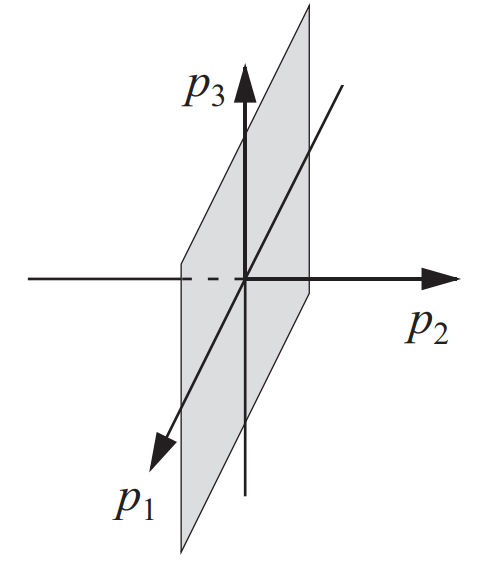
\includegraphics[width=4cm, height=4cm]{129}	
	 } 
	 
	 
	 \noindent\textbf{\Large تعامد گرام-اشمیت}
	 
	 بین تعامد و استقلال رابطه وجود دارد. می‌توان مجموعه‌ای از بردارهای مستقل را به مجموعه‌ای از بردارهای متعامد که در همان فضای برداری قرار دارند، تبدیل کرد. روش استاندارد برای تحقق این امر تعامد گرام-اشمیت نامیده می‌شود. 
	 
	 فرض کنید ما $ n $ بردار مستقل 
	 $ \mathpzc{y_1,y_2,...,y_n} $
	  را داریم. از این بردارها، $ n $ بردار متعامد 
	 $ \mathpzc{v_1,v_2,...,v_n} $
	  را به دست می‌آوریم. اولین بردار متعامد برای اولین بردار مستقل انتخاب شده است:
	 $$
	 \mathpzc{v_1=y_1} \hspace{5cm} (5.16)
	 $$
	 برای به دست آوردن بردار متعامد دوم از $ \mathpzc{y_2} $ استفاده می‌کنیم. اما بخشی از $ \mathpzc{y_2} $ را که در جهت $ \mathpzc{v_1} $ است کم کنید. عبارت زیر حاصل می‌شود:
	 $$
	 \mathpzc{v_2=y_2}-a\mathpzc{v_1} \hspace{4cm} (5.17)
	 $$
	 در جایی که $ a $ انتخاب می‌شود تا $ \mathpzc{v_2} $ متعامد با $ \mathpzc{v_1} $ باشد. این مستلزم آن است که:\\
	 
	 $$
	 \mathpzc{(v_1,v_2)=(v_1,y_2}-a\mathpzc{v_1)=(v_1,y_2)}-a\mathpzc{(v_1,v_2)}=0 \hspace{1cm} (5.18)
	 $$
	 یا
	 $$
	 a=\frac{\mathpzc{(v_1,y_2)}}{\mathpzc{(v_1,v_1)}} \hspace{3cm} (5.19)
	 $$
	 
	 بنابراین برای یافتن مؤلفه‌ی $ y_2 $ در جهت $ \mathpzc{v_1} $ و $ a\mathpzc{v_1} $، باید ضرب داخلی بین دوبردار را پیدا کنیم.
	 
	 \textbf{تصویر:}
	 ما $ a\mathpzc{v_1} $ را تصویر $ \mathpzc{y_2} $ بر روی بردار $ \mathpzc{v_1} $ می‌نامیم.
	 
	 اگر این فرایند را ادامه دهیم، $ k $امین مرحله عبارت زیر خواهد بود:
	 $$
	 \mathpzc{v}_k=\mathpzc{y}_k-\sum_{i=1}^{k-1}\frac{\mathpzc{(v}_i,\mathpzc{y}_k)}{\mathpzc{(v}_i,\mathpzc{v}_i)}\mathpzc{v}_i \hspace{3cm} (5.20)
	 $$
	 برای نشان دادن این روند، ما بردارهای مستقل زیر را در $ \Re^2 $ نظر می‌گیریم:
	 $$
	 y_1=
	 \begin{bmatrix}
	 	2 \\ 1
	 \end{bmatrix}
 	, y_2=
 	\begin{bmatrix}
 		1 \\ 2
 	\end{bmatrix}
 	\hspace{4cm} (5.21)
	 $$
	 اولین بردار متعامد، عبارت زیر خواهد بود:
	 $$
	 v_1=y_1=
	 \begin{bmatrix}
	 	2 \\ 1
	 \end{bmatrix}
 	\hspace{4cm} (5.22)
	 $$
	 دومین بردار متعامد به صورت زیر محاسبه می‌شود:
	 $$
	 v_2=y_2-\frac{v_1^Ty_2}{v_1^Tv_1}v_1=
	 \begin{bmatrix}
	 	1 \\ 2
	 \end{bmatrix}-
 	\frac{
 		\begin{bmatrix}
 			2 & 1
	 	\end{bmatrix}
	 	\begin{bmatrix}
	 		1 \\ 2
	 	\end{bmatrix}
 	}{
 		\begin{bmatrix}
 			2 & 1
 		\end{bmatrix}
 		\begin{bmatrix}
 			2 \\ 1
 		\end{bmatrix}
 	}
 	\begin{bmatrix}
 		2 \\ 1
 	\end{bmatrix}
	 =
 	\begin{bmatrix}
 		1 \\ 2
 	\end{bmatrix}
 	-
 	\begin{bmatrix}
 		1.6 \\ 1.8
 	\end{bmatrix}
 	=
 	\begin{bmatrix}
 		-0.6 \\ 1.2
 	\end{bmatrix}
 	\hspace{1cm} (5.23)
	 $$
	برای نمایش گرافیکی این فرآیند تصویر (5.1) را ببینید:
	
	
	\begin{center}
		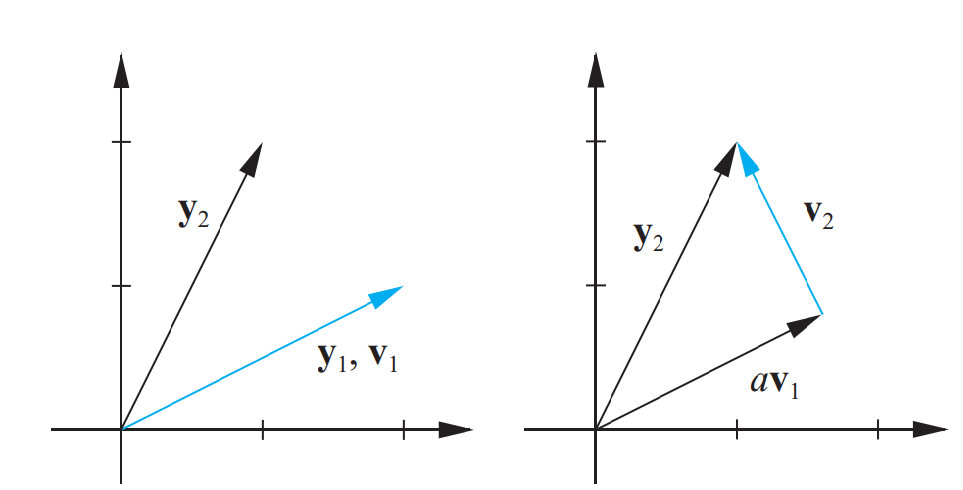
\includegraphics[width=9cm, height=4cm]{130-1}\\
		شکل (5.1) مثال تعامد گرام-اشمیت
	\end{center}
	
	ما می‌توانیم $ v_1 $ و $ v_2 $ را با تقسیم هر بردار بر روی نُرم خود به مجموعه‌ای از بردارهای متعامد (متعامد و نرمال) تبدیل کنیم.

	برای آزمایش این فرآیند متعامد سازی، از نمایشگر طراحی شبکه عصبی گرام اشمیت استفاده کنید \textbf{\lr{(nnd5gs)}}.\\
	
	\noindent\textbf{\Large بسط بردار}
	
	توجه داشته باشید که ما از فونت اسکریپت $ \mathpzc{(x)} $ برای نشان دادن بردارهای عمومی و نوع پررنگ (\textbf{\lr{x}}) برای نشان دادن بردارها در $ \Re^n $ استفاده کرده‌ایم که می‌تواند به عنوان ستون اعداد نوشته شود. در این بخش نشان خواهیم داد که بردارهای عمومی در فضاهای بردار با بعد محدود نیز می‌توانند به عنوان ستون اعداد نوشته شوند و بنابراین از برخی جهات با بردارهای $ \Re^n $ برابر هستند.
	
	\textbf{تعریف بسط بردار:}
	اگر یک فضای برداری $ X $ یک مجموعه پایه
	 $ \{\mathpzc{v_1,v_2,...,v_n}\} $
	  داشته باشد، هر 
	 $ \mathpzc{x} \in X $
	  دارای یک بردار منحصر به فرد است:
	  $$
	  \mathpzc{x}=\sum_{i=1}^{n}x_iv_i=x_1v_1+x_2v_2+...x_nv_n \hspace{3cm} (5.24)
	  $$
	  بنابراین هر بردار در فضای بردار بُعد محدود با ستونی از اعداد قابل نمایش است:
	  $$
	  \textbf{\lr{x}}=[x_1x_2...x_n]^T \hspace{3cm} (5.25)
	  $$
	  این $ \textbf{\lr{x}} $ نمایشی از بردار کلی $ \mathpzc{x} $ است.
	  البته برای تفسیر معنای $ \textbf{\lr{x}} $ لازم است مجموعه پایه را بشناسیم. اگر مجموعه پایه تغییر کند، $ \textbf{\lr{x}} $ تغییر خواهد کرد، حتی اگر بازهم همان بردار کلی $ \mathpzc{x} $ را نشان دهد. ما در بخش بعدی با جزئیات بیشتری در مورد این بحث خواهیم کرد.
	  
	  اگر بردارها در مجموعه پایه متعامد باشند
	  $ ((v_i,v_j)=0, i \neq j) $
	  ،محاسبه ضرایب در معادله بسط داده شده، بسیار آسان می‌شود. ما به راحتی ضرب داخلی $ v_j $ را با دو طرف معادله $ (5.24) $ می‌گیریم:
	  $$
	  (\mathpzc{v_j,x}) = (\mathpzc{v_j},\sum_{i=1}^{n}x_i\mathpzc{v_i}) = 
	  \sum_{i=1}^{n}x_i(\mathpzc{v_j,v_i}) = x_j(\mathpzc{v_j,v_j}) \hspace{1cm} (5.26)
	  $$
	  بنابراین ضرایب معادله بسط داده شده به روش زیر محاسبه می‌شود:
	  $$
	  x_j=\frac{(\mathpzc{v_j,x})}{(\mathpzc{v_j,v_j})} \hspace{3cm} (5.27)
	  $$
	  وقتی بردارها در مجموعه پایه متعامد نباشند، محاسبه ضرایب در بردار بسط داده شده بسیار پیچیده می‌شود. این مورد در بخش زیر پوشش داده شده است.\vspace{5cm}
	  
	  \noindent\textbf{\Large{بردارهای پایه متقابل}}
	  
	  اگر بسط بردار لازم باشد و مجموعه پایه متعامد نباشد، بردارهای پایه متقابل معرفی می‌شوند که با معادلات زیر تعریف می‌شوند:
	  $$
	  \hspace{-3.6cm}
	  \mathpzc{(r_i,v_j) = 0} \hspace{2cm} i \neq j
	  $$
	  $$
	  \hspace{2cm} = 1 \hspace{2cm} i = j \hspace{3cm} (5.28)
	  $$
	  \textbf{بردارهای پایه متقابل:}
	  وقتی که بردارهای پایه 
	  $  \mathpzc{\{v_1,v_2,...,v_n\}} $
	  و بردارهای پایه متقابل 
	  $ \mathpzc{\{r_1,r_2,...,r_n\}} $
	  باشند.
	  
	  اگر بردارها با ستون اعداد (از طریق بسط بردار) نشان داده شده باشند، و از ضرب داخلی استاندارد استفاده می‌شود
	  
	  $$
	  \mathpzc{(r_i,v_j)} = \textbf{\lr{r}}_i^T\textbf{\lr{v}}_j \hspace{3cm} (5.29)
	  $$
	  آنگاه معادله $ (5.28) $ می‌تواند به فرم ماتریسی نمایش داده شود
	  $$
	  \textbf{\lr{R}}^T\textbf{\lr{B}} = \textbf{\lr{I}} \hspace{3cm} (5.30)
	  $$
	  که
	  $$
	  \textbf{\lr{B}} = \textbf{\lr{[v}}_1 \textbf{\lr{v}}_2... \textbf{\lr{v}}_n\textbf{\lr{]}} \hspace{3cm} (5.31)
	  $$
	  $$
	  \textbf{\lr{R}} = \textbf{\lr{[r}}_1 \textbf{\lr{r}}_2... \textbf{\lr{r}}_n\textbf{\lr{]}} \hspace{3cm} (5.32)
	  $$
	  سپس $ \textbf{\lr{R}} $ می‌تواند از معادله زیر پیدا شود:
	  $$
	  \textbf{\lr{R}}^T=\textbf{\lr{B}}^{-1} \hspace{3cm} (5.33)
	  $$
	  و بردارهای پایه متقابل را می‌توان از ستون های \textbf{\lr{R}} بدست آورد.
	  
	  حال دوباره بردار بسط داده شده را در نظر بگیرید
	  $$
	  \mathpzc{x}=x_1\mathpzc{v}_1+x_2\mathpzc{v}_2+...x_n\mathpzc{v}_n \hspace{3cm} (5.34)
	  $$
	  گرفتن ضرب داخلی $ r_1 $ با دو طرف معادله \lr{(5.34)} داریم:
	  $$
	  \mathpzc{(r}_1,\mathpzc{x)}=x_1(\mathpzc{r}_1,\mathpzc{v}_1)+x_2(\mathpzc{r}_1,\mathpzc{v}_2)+...x_n(\mathpzc{r}_n,\mathpzc{v}_n) \hspace{3cm} (5.35)
	  $$
	  طبق تعریف داریم:
	  $$
	  (\mathpzc{r}_1,\mathpzc{v}_2)=(\mathpzc{r}_1,\mathpzc{v}_3)=...=(\mathpzc{r}_1,\mathpzc{v}_n)=0
	  $$
	  $$
	  (\mathpzc{r}_1,\mathpzc{v}_1)=1 \hspace{4cm} (5.36)
	  $$
	  بنابراین اولین ضریب از بسط بردار عبارت زیر خواهد بود:
	  $$
	  x_1=(\mathpzc{r}_1,\mathpzc{x}) \hspace{4cm} (5.37)
	  $$
	  و در حالت کلی
	  $$
	  x_j=(\mathpzc{r}_j,\mathpzc{x}) \hspace{4cm} (5.38)
	  $$
	  به عنوان مثال، دو بردار پایه زیر را در نظر بگیرید:
	  $$
	  \textbf{\lr{v}}_1^s=
	  \begin{bmatrix}
	  	2 \\ 1
	  \end{bmatrix}
  	  , \textbf{\lr{v}}_2^s=
  	  \begin{bmatrix}
  	  	1 \\ 2
  	  \end{bmatrix} \hspace{3cm} (5.39)
	  $$
	  فرض کنید می‌خواهیم بردار زیر را گسترش دهیم:
	  $$
	  \textbf{\lr{x}}^s=
	  \begin{bmatrix}
	  	0 \\ \frac{3}{2}
	  \end{bmatrix} \hspace{5cm} (5.40)
	  $$	  
	  از نظر دو بردار پایه.(ما از $ \mathpzc{s} $) استفاده می‌کنیم تا نشان دهیم این ستون اعداد نشان دهنده بسط بردارها از نظر پایه استاندارد در $ \Re^2 $ هستند. عناصر پایه استاندارد در شکل مجاور به عنوان بردارهای
	  $ \mathpzc{s}_1 $ 
	  و
	  $ \mathpzc{s}_2 $
	   نشان داده شده‌اند. ما باید از این نشانه صریح در این مثال استفاده کنیم، زیرا بردارها را از نظر دو مجموعه پایه متفاوت بسط خواهیم داد.)	   
	   
	   اولین قدم در بسط بردار یافتن بردارهای پایه متقابل است.\\
	   
	   \marginpar
	   {	   	
	   	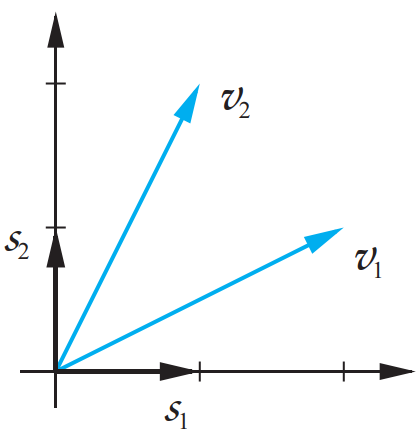
\includegraphics[width=4cm, height=4cm]{133}   
	   }
   
	   $$
	   \textbf{\lr{R}}^T=
	   \begin{bmatrix}
	   	2 & 1 \\ 1 & 2
	   \end{bmatrix}^{-1}=
   		\begin{bmatrix}
   			\frac{2}{3} & \frac{-1}{3} \\
   			\frac{-1}{3} & \frac{2}{3}
   		\end{bmatrix} \hspace{1cm}
   		\textbf{\lr{r}}_1=
   		\begin{bmatrix}
   			\frac{2}{3} \\ \frac{-1}{3}
   		\end{bmatrix} \hspace{1cm}
   		\textbf{\lr{r}}_2=
   		\begin{bmatrix}
   			\frac{-1}{3} \\ \frac{2}{3}
   		\end{bmatrix} \hspace{2cm} (5.41)
	   $$
	   اکنون می‌توان ضرایب را در بسط یافت.
	   $$
	   \hspace{-3.7cm}
	   x_1^v=\textbf{\lr{r}}_1^T\textbf{\lr{x}}^s=
	   \begin{bmatrix}
	   		\frac{2}{3} & \frac{-1}{3}
	   \end{bmatrix}
 	   \begin{bmatrix}
 	    	0 \\ \frac{3}{2}
 	   \end{bmatrix}
    	=
    	-\frac{1}{2}
	   $$
	   $$
	   x_2^v=\textbf{\lr{r}}_2^T\textbf{\lr{x}}^s=
	   \begin{bmatrix}
	   	\frac{-1}{3} & \frac{2}{3}
	   \end{bmatrix}
	   \begin{bmatrix}
	   	0 \\ \frac{3}{2}
	   \end{bmatrix}=1 \hspace{3cm} (5.42)
	   $$	   
	   یا به صورت ماتریسی	   
	   $$
	   \textbf{\lr{x}}^v=\textbf{\lr{R}}^T\textbf{\lr{x}}^s=
	   \textbf{\lr{B}}^{-1}\textbf{\lr{x}}^s=
	   \begin{bmatrix}
	   	\frac{2}{3} & \frac{-1}{3} \\
	   	\frac{-1}{3} & \frac{2}{3}
	   \end{bmatrix}
	   \begin{bmatrix}
	   	0 \\ \frac{3}{2}
	   \end{bmatrix}=
       \begin{bmatrix}
        	\frac{-1}{2} \\ 1
       \end{bmatrix} \hspace{3cm} (5.43)
	   $$	   
	   به طوری که	   
	   $$
	   \mathpzc{x}=-\frac{1}{2}\mathpzc{v}_1+1\mathpzc{v}_2 \hspace{3cm} (5.44)
	   $$
	   همانطور که در شکل \lr{5.2} نشان داده شده است.
	   \begin{center}
	   		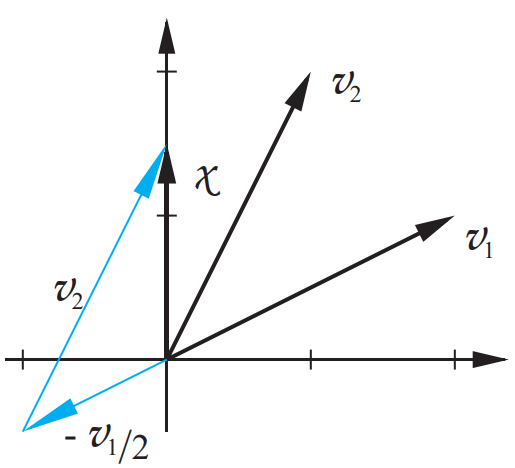
\includegraphics[width=7cm, height=6cm]{134}
	   		
	   		شکل \lr{5.2} بسط برداری
	   \end{center}
   توجه داشته باشید که اکنون دو بسط برداری متفاوت برای $ \mathpzc{x} $ داریم، که به صورت
   	$ \textbf{\lr{x}}^s $
   	و
   	$ \textbf{\lr{x}}^v $
   	نشان داده شده است. به عبارت دیگر
   	$$
   	\mathpzc{x}=0\mathpzc{s}_1+\frac{3}{2}\mathpzc{s}_2=
   	-\frac{1}{2}\mathpzc{v}_1+1\mathpzc{v}_2 \hspace{3cm} (5.42)
   	$$
   	هنگامی که ما یک بردار کلی را به عنوان ستونی از اعداد نشان می‌دهیم ، باید بدانیم که از چه مجموعه پایه‌ای برای بسط استفاده شده است. در این متن فرض کنید که از مجموعه پایه استاندارد استفاده شده است.
   	
   	معادله \lr{5.43} دو نمایش متفاوت از $ \mathpzc{x} $ را نشان می‌دهد،
   	$ \textbf{\lr{x}}^v=\textbf{\lr{B}}^{-1}\textbf{\lr{x}}^s $
   	این عملیات که تغییر پایه نامیده می‌شود، در فصل‌های بعدی برای تجزیه و تحلیل عملکرد برخی شبکه‌های عصبی بسیار مهم خواهد شد.
   
   	برای آزمایش این فرآیند بسط بردار، از نمایشگر طراحی شبکه عصبی پایه‌های متقابل استفاده کنید \textbf{\lr{(nnd5rb)}}.
   	\vspace{10cm}
   	
   	\noindent\textbf{\Large{خلاصه نتایج}}
   	\hrule \vspace{0.3cm}
   	\textbf{\large{فضاهای برداری خطی}}
   	
   	\textbf{فضای برداری}:
   	 یک فضای بردار خطی، مجموعه‌ای از عناصر (بردارها) تعریف شده در یک میدان اسکالر است، که شرایط زیر را برآورده می‌کند:
   	
   	1.	عملیاتی به نام جمع برداری به گونه ای تعریف می شود که اگر
   	$ \mathpzc{x} \in X $ ($ \mathpzc{x} $
   	یک عنصر از \lr{X} است) و
   	$ \mathpzc{y} \in X $،
   	آنگاه 
   	$ \mathpzc{x+y} \in X $.\\
   	
   	2. $ \mathpzc{x+y=y+x} $\\
   	
   	3. $ \mathpzc{(x+y)+z=x+(y+z)} $\\
   	
   	4.	یک بردار منحصر به فرد وجود دارد:
   	$ 0 \in X $
   	که بردار صفر نامیده می‌شود، به طوری که
   	$ \mathpzc{x+0=x} $ 
   	برای همه
   	$ \mathpzc{x} \in X $.\\
   	
   	5. برای هر بردار 
   	$ \mathpzc{x} \in X $
   	یک بردار یکتا در $ X $ وجود دارد که
   	$ \mathpzc{-x} $
   	نامیده می‌شود، مانند 
   	$ \mathpzc{x+(-x)=0} $.\\
   	
   	6. عملیاتی به نام ضرب تعریف می‌شود به این صورت که برای همه اسکالرها 
   	$ a \in F $
   	و همه‌ی بردارها
   	$ \mathpzc{x} \in X $ و $ a\mathpzc{x} \in X $.\\
   	
   	7. برای هر 
   	$ \mathpzc{x} \in X $
   	و
   	$ 1\mathpzc{x}=\mathpzc{x} $
   	(برای اسکالر 1)\\
   	
   	8. برای دو اسکالر $ a \in F $ و $ b \in F $ و هر 
   	$ \mathpzc{x} \in X $ ، $ a(b\mathpzc{x})=(ab)\mathpzc{x} $.\\
   	
   	9. $ (a+b)\mathpzc{x}=a\mathpzc{x}+b\mathpzc{x} $\\
   	
   	10. $ a(\mathpzc{x+y}) = a\mathpzc{x}+a\mathpzc{y} $\\
   	
   	\textbf{\large{مستقل خطی}}
   	
   	$ n $ بردار
   	$ \mathpzc{\{x_1, x_2, ... ,x_n\}} $
   	را در نظر بگیرید. اگر $ n $ اسکالر
   	$ a_1, a_2, ... ,a_n $
   	وجود داشته باشد، حداقل یکی از آنها غیر صفر است؛ مانند:
   	
   	$$
   	a_1\mathpzc{x_1} + a_2\mathpzc{x_2} + ... + a_n\mathpzc{x_n} = 0
   	$$
   	
   	بنابراین 
   	$ \mathpzc{\{ x_i \}} $
   	وابسته خطی هستند.\\\\
   	
   	\textbf{\large{پدید آوردن یک فضا}}
   	
   	فرض کنیم $ X $ فضای برداری خطی باشد و $ \{ u_1,u_2,...,u_n \} $ زیرمجموعه بردارهای عمومی در $ X $ باشد. این زیرمجموعه $ X $ را پدید می‌آورد اگر و فقط اگر برای هر بردار 
   	$ \mathpzc{x} \in X $
   	اسکالرهای
   	$ \mathpzc{x_1,x_2,...,x_n} $
   	وجود داشته باشد، به طوری که
   	$ \mathpzc{x} = x_1u_1+x_2u_2+...+x_mu_m $.\\
   	
   	
   	\textbf{\large{ضرب داخلی}}
   	
   	هر عملکرد اسکالر $ x $ و $ y $ را می‌توان به عنوان یک ضرب داخلی تعریف کرد. مشروط بر اینکه خواص زیر برآورده شود:
   	
   	1. $ \mathpzc{(x,y)=(y,x)} $
   	
   	2. $ (\mathpzc{x},a\mathpzc{y}_1+b\mathpzc{y}_2)=a(\mathpzc{x,y_1})+b(\mathpzc{x,y_2}) $
   	
   	3. $ \mathpzc{(x,x)} \geq 0 $،
   	زمانی برابر است اگر و فقط اگر $ \mathpzc{x} $ بردار صفر است.\\
   	
   	\textbf{\large{نُرم}}
   	
   	تابع اسکالر 
   	$ \Vert \mathpzc{x} \Vert$
   	نُرم می‌نامیم اگر شرایط زیر را داشته باشد:
   	
   	1. $ \Vert \mathpzc{x} \Vert \geq 0 $
   	
   	2. $ \Vert \mathpzc{x} \Vert = 0 $ اگر و فقط اگر $ \mathpzc{x}=0 $.	
   	
   	3. $ \Vert a\mathpzc{x} \Vert = \vert a \vert \Vert \mathpzc{x} \Vert $ برای اسکالر $ a $
   	
   	4. $ \Vert \mathpzc{x+y} \Vert \leq \Vert \mathpzc{x} \Vert + \Vert \mathpzc{y} \Vert $\\
   	
   	\textbf{\large{زاویه}}
   	
   	زاویه $ \theta $ بین دو بردار $ \mathpzc{x} $ و $ \mathpzc{y} $ به صورت زیر تعریف می‌شود:
   	
   	$$
   	\cos \theta = \frac{\mathpzc{(x,y)}}{\Vert \mathpzc{x} \Vert \Vert \mathpzc{y} \Vert}
   	$$
   	
   	\textbf{\large{تعامد}}
   	
   	دو بردار $ \mathpzc{x,y} \in X $ متعامد هستند اگر $ \mathpzc{(x,y)}=0 $.\\
   	
   	\textbf{\large{تعامد گرام-اشمیت}}
   	
   	فرض کنید ما $ n $ بردار مستقل 
   	$ \mathpzc{y_1,y_2,...,y_n} $
   	را داریم. از این بردارها، $ n $ بردار متعامد 
   	$ \mathpzc{v_1,v_2,...,v_n} $
   	را به دست می‌آوریم.
   	$$
   	\mathpzc{v_1=y_1}
   	$$
   	
   	$$
   	\mathpzc{v}_k=\mathpzc{y}_k-\sum_{i=1}^{k-1}\frac{\mathpzc{(v}_i,\mathpzc{y}_k)}{\mathpzc{(v}_i,\mathpzc{v}_i)}\mathpzc{v}_i
   	$$
   	که
   	$$
   	\frac{\mathpzc{(v}_i,\mathpzc{y}_k)}{\mathpzc{(v}_i,\mathpzc{v}_i)}\mathpzc{v}_i
   	$$
   	تصویر 
   	$ \mathpzc{y}_k $
   	 روی
    $ \mathpzc{v}_i $
     است.\\
     
     \textbf{\large{بسط بردار}}
     $$
     \mathpzc{x}=\sum_{i=1}^{n}x_iv_i=x_1v_1+x_2v_2+...x_nv_n
     $$
     بردارهای متعامد
     $$
     x_j=\frac{(\mathpzc{v_j,x})}{(\mathpzc{v_j,v_j})}
     $$
     
     \textbf{\large{بردارهای پایه متقابل}}
     $$
     \mathpzc{(r_i,v_j) = 0} \hspace{2cm} i \neq j
     $$
     $$
     \hspace{1.4cm} = 1 \hspace{2cm} i = j
     $$
     $$
     \hspace{-1.1cm} x_j=(\mathpzc{r}_j,\mathpzc{x}).
     $$
     برای محاسبه بردارهای پایه متقابل:
      $$
     \textbf{\lr{B}} = \textbf{\lr{[v}}_1 \textbf{\lr{v}}_2... \textbf{\lr{v}}_n\textbf{\lr{]}},
     $$
     $$
     \textbf{\lr{R}} = \textbf{\lr{[r}}_1 \textbf{\lr{r}}_2... \textbf{\lr{r}}_n\textbf{\lr{]}},
     $$
     $$
     \textbf{\lr{R}}^T=\textbf{\lr{B}}^{-1}.
     $$
     فرم ماتریسی:
     $$
     \textbf{\lr{x}}^v=\textbf{\lr{B}}^{-1}\textbf{\lr{x}}^s
     $$
     \vspace{10cm}
     
     \noindent\textbf{\Large{مسائل حل شده}}
     \hrule \vspace{0.3cm}
     
     \hspace{-2cm}\textbf{\lr{:P5.1}}
     \textbf
     {
     	شبکه تک نورونی پرسپترون را در نظر بگیرید که در شکل \lr{P5.1} نشان داده شده است. از فصل 3 به یاد بیاورید (معادله (3.6) را ببینید) مرز تصمیم گیری برای این شبکه توسط 
     	$ \textbf{\lr{Wp}}+b=0 $
     	تعیین شده است. اگر $ b = 0 $ نشان دهید که مرز تصمیم یک فضای بردار است.
     } 
     
      \begin{center}
      	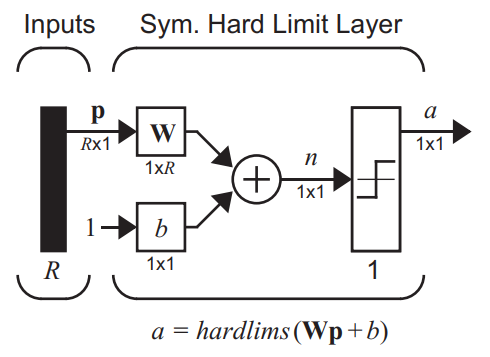
\includegraphics[width=8cm, height=6cm]{138}
      	
      	شکل \lr{P5.1} پرسپترون تک نرون
      \end{center}
  برای اینکه یک فضای بردار باشد، مرز باید ده شرط ارائه شده در ابتدای این فصل را برآورده کند. شرط 1 ایجاب می‌کند که وقتی دو بردار را با هم جمع می‌کنیم جمع در فضای بردار باقی بماند. بگذارید
   $ \textbf{\lr{p}}_1 $
    و 
   $ \textbf{\lr{p}}_2 $
    دو بردار در مرز تصمیم گیری باشید. برای اینکه در مرز باشند شرایط زیر باید برآورده شود:
    $$
    \textbf{\lr{Wp}}_1=0 \hspace{1cm}
    \textbf{\lr{Wp}}_2=0.
    $$
    اگر این دو معادله را باهم جمع کنیم داریم:
    $$
    \textbf{\lr{W}}{(\textbf{\lr{p}}_1+\textbf{\lr{p}}_2)}=0
    $$
    بنابراین این جمع نیز روی مرز تصمیم گیری خواهد بود.\\
    
    شرایط 2 و 3 به وضوح برآورده شده است. شرط 4 ایجاب می‌کند که بردار صفر روی مرز باشد. از آنجا که
    $ \textbf{\lr{W0}} = 0 $،
     بردار صفر روی مرز تصمیم گیری است. شرط 5 نشان می‌دهد که اگر \textbf{\lr{p}} روی مرز \textbf{\lr{-p}} باشد، پس باید روی مرز نیز باشد. اگر \textbf{\lr{p}} روی مرز باشد، سپس:
     $$
     \textbf{\lr{Wp}}=0
     $$
     اگر دو طرف معادله را در \lr{-1} ضرب کنیم، داریم:
     $$
     \textbf{\lr{W}}(-\textbf{\lr{p}})=0
     $$
     بنابراین شرط 5 نیز برآورده می‌شود.
     
     اگر برای هر \textbf{\lr{p}} روی مرز،
     $ a\textbf{\lr{p}} $
      نیز روی مرز باشد، شرط 6 برآورده خواهد شد. این را می توان به همان روش 5 نشان داد. کافی است هر دو طرف معادله را به جای 1 در $ a $ ضرب کنید.
      $$
      \textbf{\lr{W}}(a\textbf{\lr{p}})=0
      $$
      شرایط 7 تا 10 به وضوح برآورده شده است. بنابراین مرز تصمیم گیرندی پرسپترون یک فضای برداری است.\\
      
      \hspace{-2cm}\textbf{\lr{P5.2}}
      \textbf
      {
      	نشان دهید که مجموعه \lr{Y} توابع پیوسته غیرمنفی ($ f(t) \geq 0 $) یک فضای بردار نیست.
      }
      
      این مجموعه چندین شرط مورد نیاز برای یک فضای بردار را نقض می‌کند. به عنوان مثال، هیچ بردار منفی وجود ندارد، بنابراین شرط 5 نمی‌تواند برآورده شود. همچنین، شرط 6 را در نظر بگیرید. تابع $ f(t)=|t| $ عضوی از \lr{Y} است. می‌گذاریم $ a=-2 $. سپس:
      $$
      af(2)=-2|2|=-4 < 0.
      $$
      بنابراین $ af(t) $ عضو \lr{Y} نیست، و شرط 6 برآورده نمی‌شود.\\
      
      \hspace{-2cm}\textbf{\lr{P5.3}}
      \textbf
      {
      	کدام یک از بردارهای زیر مستقل هستند؟ بعد فضای برداری را که توسط هر مجموعه پدید آمده است را پیدا کنید.
      }  
  	  $$
  	  \textbf{\lr{i.}}
  	  \begin{bmatrix}
  	  	1 \\ 1 \\ 1
  	  \end{bmatrix}
	  \hspace{1cm}
   	  \begin{bmatrix}
   	    	1 \\ 0 \\ 1
   	  \end{bmatrix}
      \hspace{1cm}
      \begin{bmatrix}
        	1 \\ 2 \\ 1
      \end{bmatrix}
  	  $$
  	  $$
  	  \textbf{\lr{ii.}} \sin t \hspace{1cm} \cos t \hspace{1cm} 2\cos (t+\frac{\pi}{4})
  	  $$
  	  $$
  	  \textbf{\lr{iii.}}
  	  \begin{bmatrix}
  	  	1 \\ 1 \\ 1 \\ 1
  	  \end{bmatrix}
      \begin{bmatrix}
      	1 \\ 0 \\ 1 \\ 1
      \end{bmatrix}
	  \begin{bmatrix}
	  	1 \\ 2 \\ 1 \\ 1
	  \end{bmatrix}
  	  $$
  	  \textbf{\lr{.i }}
  	  ما می‌توانیم این مشکل را از چند طریق حل کنیم. اول، فرض کنیم بردارها وابسته باشند. سپس می‌توانیم بنویسیم
  	  $$
  	  a_1
  	  \begin{bmatrix}
  	  	1 \\ 1 \\ 1
  	  \end{bmatrix}
      a_2
      \begin{bmatrix}
      	1 \\ 0 \\ 1
      \end{bmatrix}
 	  a_3
 	  \begin{bmatrix}
 	  	1 \\ 2 \\ 1
 	  \end{bmatrix}
   	  =
   	  \begin{bmatrix}
   	  	0 \\ 0 \\ 0
   	  \end{bmatrix}.
  	  $$
  	  اگر بتوانیم ضرایب را پیدا کنیم و همه آنها صفر نباشند، بردارها وابسته هستند. با بازرسی می‌توان دریافت که اگر بگذاریم
  	   $ a_1 = 2 , a_2 = -1 , a_3 = -1 $
  	    باشد، آنگاه این معادله برآورده می‌شود. بنابراین بردارها وابسته هستند.\\
  	    
  	    رویکرد دیگر، هنگامی که $ n $ بردار در $ \Re^n $ داشته باشیم، می‌توانیم معادله فوق را به صورت ماتریس بنویسیم:
  	    $$
  	    \begin{bmatrix}
  	    	1 & 1 & 1
  	    	\\
  	    	1 & 0 & 2
  	    	\\
  	    	1 & 1 & 1
  	    \end{bmatrix}  	    
  	    \begin{bmatrix}
  	    	a_1 \\ a_2 \\ a_3
  	    \end{bmatrix}
      =
  	    \begin{bmatrix}
  	    	0 \\ 0 \\ 0
  	    \end{bmatrix}
  	    $$
  	    اگر ماتریس در این معادله معکوس داشته باشد، در اینصورت نیاز به صفر بودن تمام ضرایب است. بنابراین بردارها مستقل هستند. اگر ماتریس منفرد باشد (معکوس نداشته باشد)، یک ضریب غیر صفر کار خواهد کرد، و بردارها وابسته هستند. بنابراین، آزمایش ایجاد یک ماتریس با استفاده از بردارها به عنوان ستون است. اگر دترمینان ماتریس صفر باشد (ماتریس منفرد)، بردارها وابسته هستند. در غیر این صورت مستقل هستند. با استفاده از بسط لاپلاس \lr{[Brog91]} در ستون اول، دترمینان این ماتریس برابر:
  	    $$
  	    \begin{vmatrix}
  	    	1 & 1 & 1
  	    	\\
  	    	1 & 0 & 2
  	    	\\
  	    	1 & 1 & 1
  	    \end{vmatrix}  	    
      	=1
  	    \begin{vmatrix}
  	    	0 & 2 \\ 1 & 1
  	    \end{vmatrix}
  	    +(-1)
  	    \begin{vmatrix}
  	    	1 & 1 \\ 1 & 1
  	    \end{vmatrix}
      	+1
      	\begin{vmatrix}
      		1 & 1 \\ 0 & 2
      	\end{vmatrix}
      	=-2+0+2=0
  	    $$
  	    بنابراین بردارها وابسته هستند.
  	    
  	    بعد فضایی که به وسیله‌ی بردارها پدید آمد برابر 2 است، زیرا می‌توان هر دو بردار را به صورت مستقل نشان داد.\\
  	    
  	    \textbf{\lr{.ii }}
  	    با استفاده از برخی اتحادهای مثلثاتی می‌توانیم بنویسیم
  	   $$
  	   \cos (t+\frac{\pi}{4})=
  	   \frac{-1}{\sqrt 2}\sin t+\frac{1}{\sqrt 2}\cos t.
  	   $$ 
  	   بنابراین بردارها وابسته هستند. بعد فضای بردار که توسط دو بردار پدید آمده، برابر دو است، زیرا هیچ ترکیب خطی از آن نیست و به طور یکسان صفر است.\\
  	   
  	   \textbf{\lr{.iii }}
  	   این شبیه قسمت \lr{(i)} است، با این تفاوت که تعداد بردارها کمتر از اندازه فضای برداری است که از آنها کشیده می شود(سه بردار در $ \Re^4 $). در این حالت ماتریس ساخته شده از بردارها مربع نخواهد بود، بنابراین ما قادر به محاسبه یک دترمینان نخواهیم بود. با این حال، ما می‌توانیم از چیزی به نام \lr{Gramian [Brog91]} استفاده کنیم. این دترمینان ماتریسی است که عنصر \lr{i} و \lr{j} ضرب داخلی بردار \lr{i} و بردار \lr{j} است. بردارها وابسته هستند اگر و فقط اگر گرامیان صفر باشد.
  	   
  	   برای مسئله ما گرامیان به صورت زیر خواهد بود
  	   $$
  	   G=
  	   \begin{vmatrix}
	  	   	(\textbf{\lr{x}}_1,\textbf{\lr{x}}_1) & 
	  	   	(\textbf{\lr{x}}_1,\textbf{\lr{x}}_2) &
	  	   	(\textbf{\lr{x}}_1,\textbf{\lr{x}}_3) \\
	  	   	(\textbf{\lr{x}}_2,\textbf{\lr{x}}_1) &
	  	   	(\textbf{\lr{x}}_2,\textbf{\lr{x}}_2) &
	  	   	(\textbf{\lr{x}}_2,\textbf{\lr{x}}_3) \\
	  	   	(\textbf{\lr{x}}_3,\textbf{\lr{x}}_1) &
	  	   	(\textbf{\lr{x}}_3,\textbf{\lr{x}}_2) &
	  	   	(\textbf{\lr{x}}_3,\textbf{\lr{x}}_3)
  	   \end{vmatrix},
       $$
       که
       $$
       \textbf{\lr{x}}_1=
       \begin{bmatrix}
	       	1 \\ 1 \\ 1 \\ 1
       \end{bmatrix}
   	   \textbf{\lr{x}}_2=
   	   \begin{bmatrix}
   	   	1 \\ 0 \\ 1 \\ 1
   	   \end{bmatrix}
       \textbf{\lr{x}}_3=
       \begin{bmatrix}
       	1 \\ 2 \\ 1 \\ 1
       \end{bmatrix}
  	   $$
  	   بنابراین
  	   $$
  	   G=
  	   \begin{vmatrix}
	  	   	4 & 3 & 5 \\
	  	   	3 & 3 & 3 \\
	  	   	5 & 3 & 7 \\	  	   	
  	   \end{vmatrix}
       =4
       \begin{vmatrix}
	       	3 & 3 \\
	       	3 & 7
       \end{vmatrix}
   	   +(-3)
   	   \begin{vmatrix}
	   	   	3 & 5 \\
	   	   	3 & 7
   	   \end{vmatrix}
       +5
       \begin{vmatrix}
	       	3 & 5 \\
	       	3 & 3
       \end{vmatrix}
   	   =48-18-30=0
  	   $$
  	   همچنین با یادداشت زیر می‌توانیم وابسته بودن این بردارها را نشان دهیم:
  	   $$
  	   2
  	   \begin{bmatrix}
	  	   	1 \\ 1 \\ 1 \\ 1
  	   \end{bmatrix}
       -1
       \begin{bmatrix}
       	1 \\ 0 \\ 1 \\ 1
       \end{bmatrix}
   	   -1
   	   \begin{bmatrix}
   	   	1 \\ 2 \\ 1 \\ 1
   	   \end{bmatrix}
       =
       \begin{bmatrix}
       	0 \\ 0 \\ 0 \\ 0
       \end{bmatrix}
  	   $$
  	   بنابراین ابعاد فضا باید کمتر از 3 باشد. می‌توان نشان داد که
  	   $ \textbf{\lr{x}}_1 $
  	    و
  	    $ \textbf{\lr{x}}_2 $
  	     مستقل هستند، زیرا
  	     $$
  	     G=
  	     \begin{vmatrix}
	  	     4 & 3 \\
	  	     3 & 3
  	     \end{vmatrix}
       	 =4 \neq 0.
  	     $$
  	     بنابراین بعد فضا 2 است.\\
  	     
  	     \hspace{-2cm}\textbf{\lr{P5.4}}
  	     \textbf
  	     {
  	     	از فصل 3 و 4 به یاد بیاورید که از پرسپترون‌های تک لایه فقط می‌توان الگوهایی را تشخیص داد که به صورت خطی قابل تفکیک هستند (می‌توان آنها را با یک مرز خطی از هم جدا کرد - شکل 3.3 را ببینید). اگر دو الگو به طور خطی قابل تفکیک باشند، آیا همیشه از نظر خطی مستقل هستند؟
  	     }
       
       
  	     نه، این دو مفهوم غیر مرتبط هستند. مثال ساده زیر را درنظر بگیرید. دو پرسپترون ورودی را که در شکل \lr{P5.2} نشان داده شده است در نظر بگیرید. 
  	     
  	     فرض کنید می‌خواهیم دو بردار را از هم جدا کنیم
  	     $$
  	     \textbf{\lr{P}}_1=
  	     \begin{bmatrix}
  	     	0.5 \\ 0.5
  	     \end{bmatrix}
       	 \hspace{2cm}
       	 \textbf{\lr{P}}_2=
       	 \begin{bmatrix}
       	 	1.5 \\ 1.5
       	 \end{bmatrix}
  	     $$
  	     اگر وزن‌ها و انحرافات را به اینصورت انتخاب کنیم
  	     $ w_{11}=1, w_{12}=1 $
  	     و
  	     $ b=-2 $،
  	      پس مرز تصمیم 
  	     $ (\textbf{\lr{Wp}}+b=0) $
  	       در شکل سمت چپ نشان داده شده است. واضح است که این دو بردار از نظر خطی قابل تفکیک هستند. با این حال، آنها از نظر خطی مستقل نیستند، زیرا   	         	       
  	       $ \textbf{\lr{P}}_2=3\textbf{\lr{P}}_1 $.
  	       \marginpar
  	       {
  	       		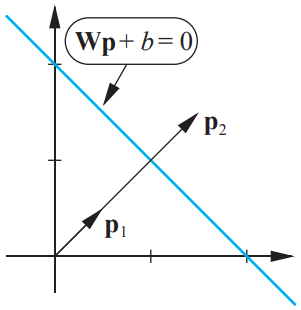
\includegraphics[width=4cm, height=4cm]{142-2}
  	       }
  	       \begin{center}
	  	       	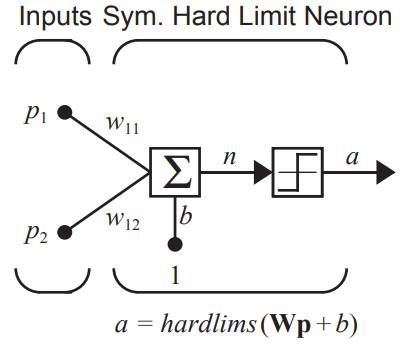
\includegraphics[width=7cm, height=6cm]{142}
	  	       	
	  	       	شکل \lr{P5.2} پرسپترون دو ورودی
  	       \end{center}
         
         \hspace{-2cm}\textbf{\lr{P5.5}}
         \textbf
         {
         	با استفاده از بردارهای پایه زیر، یک مجموعه متعامد را با استفاده از حالت تعاملی گرام-اشمیت پیدا کنید.
         }         
         $$
         \textbf{\lr{y}}_1=
         \begin{bmatrix}
         	1 \\ 1 \\ 1
         \end{bmatrix}
         \textbf{\lr{y}}_2=
         \begin{bmatrix}
         	1 \\ 0 \\ 0
         \end{bmatrix}
         \textbf{\lr{y}}_3=
         \begin{bmatrix}
         	0 \\ 1 \\ 0
         \end{bmatrix}
         $$
         مرحله 1.
         $$
         \textbf{\lr{v}}_1=\textbf{\lr{y}}_1=
         \begin{bmatrix}
         	1 \\ 1 \\ 1
         \end{bmatrix}
         $$
         مرحله 2.
         $$
         \textbf{\lr{v}}_2=\textbf{\lr{y}}_2-
         \frac{\textbf{\lr{v}}_1^T\textbf{\lr{y}}_2}
         {\textbf{\lr{v}}_1^T\textbf{\lr{v}}_1}
         \textbf{\lr{v}}_1=
         \begin{bmatrix}
         	1 \\ 0 \\ 0
         \end{bmatrix}
     	 -
     	 \frac
     	 {
     	 	\begin{bmatrix}
     	 		1 & 1 & 1
     	 	\end{bmatrix}
      		\begin{bmatrix}
      			1 \\ 0 \\ 0
      		\end{bmatrix}
     	 }
     	 {
     	 	\begin{bmatrix}
     	 		1 & 1 & 1
     	 	\end{bmatrix}
     	 	\begin{bmatrix}
     	 		1 \\ 1 \\ 1
     	 	\end{bmatrix}
     	 }
      	 \begin{bmatrix}
      	 	1 \\ 1 \\ 1
      	 \end{bmatrix}
       	 =
       	 \begin{bmatrix}
       	 	1 \\ 0 \\ 0
       	 \end{bmatrix}
         -
       	 \begin{bmatrix}
       	 	1/3 \\ 1/3 \\ 1/3
       	 \end{bmatrix}
         =
         \begin{bmatrix}
         	2/3 \\ -1/3 \\ -1/3
         \end{bmatrix}
         $$
         مرحله 3.
         $$
         \textbf{\lr{v}}_3=\textbf{\lr{y}}_3-
         \frac{\textbf{\lr{v}}_1^T\textbf{\lr{y}}_3}
         {\textbf{\lr{v}}_1^T\textbf{\lr{v}}_1}
         \textbf{\lr{v}}_1-
         \frac{\textbf{\lr{v}}_2^T\textbf{\lr{y}}_3}
         {\textbf{\lr{v}}_2^T\textbf{\lr{v}}_2}
         \textbf{\lr{v}}_2
         $$
         $$
         \textbf{\lr{v}}_3=
         \begin{bmatrix}
         	0 \\ 1 \\ 0
         \end{bmatrix}
         -
         \frac
         {
         	\begin{bmatrix}
         		1 & 1 & 1
         	\end{bmatrix}
         	\begin{bmatrix}
         		0 \\ 1 \\ 0
         	\end{bmatrix}
         }
         {
         	\begin{bmatrix}
         		1 & 1 & 1
         	\end{bmatrix}
         	\begin{bmatrix}
         		1 \\ 1 \\ 1
         	\end{bmatrix}
         }
         \begin{bmatrix}
         	1 \\ 1 \\ 1
         \end{bmatrix}
     	 -
     	 \frac
     	 {
     	 	\begin{bmatrix}
     	 		2/3 & -1/3 & -1/3
     	 	\end{bmatrix}
     	 	\begin{bmatrix}
     	 		0 \\ 1 \\ 0
     	 	\end{bmatrix}
     	 }
     	 {
     	 	\begin{bmatrix}
     	 		2/3 & -1/3 & -1/3
     	 	\end{bmatrix}
     	 	\begin{bmatrix}
     	 		2/3 \\ -1/3 \\ -1/3
     	 	\end{bmatrix}
     	 }
     	 \begin{bmatrix}
     	 	2/3 \\ -1/3 \\ -1/3
     	 \end{bmatrix}
      	 $$
      	 $$
         \textbf{\lr{v}}_3=
         \begin{bmatrix}
         	0 \\ 1 \\ 0
         \end{bmatrix}
         -
         \begin{bmatrix}
         	1/3 \\ 1/3 \\ 1/3
         \end{bmatrix}
     	 -
     	 \begin{bmatrix}
     	 	-1/3 \\ 1/6 \\ 1/6
     	 \end{bmatrix}
         =
         \begin{bmatrix}
         	0 \\ 1/2 \\ -1/2
         \end{bmatrix}
         $$\\
         
         \hspace{-2cm}\textbf{\lr{P5.6}}
         \textbf
         {
         	فضای بردار تمام چند جمله‌ای های تعریف شده را در بازه
         	$ [1- , 1]  $ در نظر بگیرید. نشان دهید 
         	$ (\mathpzc{x,y})=\int_{-1}^{1}\mathpzc{x(t)y(t)}dt $          
         	یک ضرب داخلی معتبر است.
         }         
         یک محصول داخلی باید دارای خواص زیر باشد.
         
         1. $ (\mathpzc{x,y})=(\mathpzc{y,x}) $
         $$
         (\mathpzc{x,y})=\int_{-1}^1\mathpzc{x(t)y(t)dt}=
         \int_{-1}^1\mathpzc{y(t)x(t)dt}=(\mathpzc{y,x})
         $$
         
         2. $ (\mathpzc{x,}a\mathpzc{y}_1+b\mathpzc{y}_2)=
         a(\mathpzc{x,y}_1)+b(\mathpzc{x,y}_2) $
         $$
         (\mathpzc{x,}a\mathpzc{y}_1+b\mathpzc{y}_2)=
         \int_{-1}^1\mathpzc{x(t)}(a\mathpzc{y}_1(t)+b\mathpzc{y}_2(t))dt=
         a\int_{-1}^{1}\mathpzc{x(t)y}_1(t)dt+
         b\int_{-1}^{1}\mathpzc{x(t)y}_2(t)dt                 
         $$
         $$
         =a(\mathpzc{x,y}_1)+b(\mathpzc{x,y}_2) 
         $$
         
         3. $ (\mathpzc{x.x}) \geq 0 $،
         جایی که برابری برقرار است اگر و فقط اگر $ \mathpzc{x} $ بردار صفر باشد.
         $$
         (\mathpzc{x,x})=\int_{-1}^{1}\mathpzc{x(t)x(t)dt}=
         \int_{-1}^{1}\mathpzc{x}^2(t)dt \geq 0
         $$
         برابری برقرار است اگر و فقط اگر 
         $ \mathpzc{x(t)}=0 $
         برای
         $ -1 \leq t \leq 1 $،
         که بردار صفر است.\\
         
         \hspace{-2cm}\textbf{\lr{P5.7}}
         \textbf
         {
دو بردار از فضای بردار توصیف شده در مسئله قبلی (چند جمله‌ای های تعریف شده در فاصله
 $ [-1 , 1] $) 
  $ 1+t $ و
  $ 1-t $
   هستند. بر اساس این دو بردار، یک مجموعه بردار متعامد پیدا کنید.
         }
         مرحله 1.
         $$
         \mathpzc{v}_1=\mathpzc{y}_1=1+t
         $$
         مرحله 2.
         $$
         \mathpzc{v_2}=\mathpzc{y_2}-
         \frac{(\mathpzc{v_1,y_2})}
         {\mathpzc{v_1,v_1}}\mathpzc{v_1}
         $$
         که
         $$
         (\mathpzc{v_1,y_2})=
         \int_{-1}^{1}(1+t)(1-t)dt=\left. \left(t-\frac{t^3}{3}\right)\right|_{-1}^{1}=
         \left (\frac{2}{3}\right)-
         \left (\frac{-2}{3}\right)=\frac{4}{3}
         $$
         $$
         (\mathpzc{v_1,v_1})=
         \int_{-1}^{1}(1+t)^2dt=\left. \left(\frac{1+t^3}{3}\right)\right|_{-1}^{1}=
         \left (\frac{8}{3}\right)-
         (0)=\frac{8}{3}.
         $$
         بنابراین
         $$
         \mathpzc{v_2}=(1-t)-\frac{4/3}{8/3}(1+t)=\frac12-\frac32t.
         $$
         \\
         \hspace{-2cm}\textbf{\lr{P5.8}}
         \textbf
         {
         	$ \textbf{\lr{x}}=
         	\begin{bmatrix}
         		6 & 9 & 9
         	\end{bmatrix}^T $
         	 را از نظر مجموعه پایه زیر گسترش دهید.
         }
     	 
     	 $$
     	 \textbf{\lr{v}}_1=
     	 \begin{bmatrix}
     	 	1 \\ 1 \\ 1
     	 \end{bmatrix}
     	 \textbf{\lr{v}}_2=
     	 \begin{bmatrix}
     	 	1 \\ 2 \\ 3
     	 \end{bmatrix}
     	 \textbf{\lr{v}}_3=
     	 \begin{bmatrix}
     	 	1 \\ 3 \\ 2
     	 \end{bmatrix}
     	 $$
     	 اولین قدم محاسبه بردارهای پایه متقابل است.
     	 $$
     	 \textbf{\lr{B}}=
     	 \begin{bmatrix}
     	 	1 & 1 & 1 \\
     	 	1 & 2 & 3 \\
     	 	1 & 3 & 2
     	 \end{bmatrix}
         \textbf{\lr{B}}^{-1}=
      	 \begin{bmatrix}
      	 	\frac53 & -\frac13 & -\frac13 \\
      	 	-\frac13 & -\frac13 & \frac23 \\
      	 	-\frac13 & \frac23 & -\frac13
      	 \end{bmatrix}
     	 $$
     	 ردیف های 
     	 $ \textbf{\lr{B}}^{-1} $
     	 را جدا می‌کنیم،
     	 $$
     	 \textbf{\lr{r}}_1=
     	 \begin{bmatrix}
     	 	5/3 \\ -1/3 \\ -1/3
     	 \end{bmatrix}
      	 \textbf{\lr{r}}_2=
      	 \begin{bmatrix}
      	 	-1/3 \\ -1/3 \\ 2/3
      	 \end{bmatrix}
       	 \textbf{\lr{r}}_3=
       	 \begin{bmatrix}
       	 	-1/3 \\ 2/3 \\ -1/3
       	 \end{bmatrix}
     	 $$
     	 ضرایب در بسط محاسبه می‌شود
     	 $$
     	 x_1^v=\textbf{\lr{r}}_1^T\textbf{\lr{x}}=
     	 \begin{bmatrix}
     	 	\frac53 & \frac{-1}3 & \frac{-1}3
     	 \end{bmatrix}
      	 \begin{bmatrix}
      	 	6 \\ 9 \\ 9
      	 \end{bmatrix}
       	 =4
     	 $$
     	 $$
     	 x_2^v=\textbf{\lr{r}}_2^T\textbf{\lr{x}}=
     	 \begin{bmatrix}
     	 	\frac{-1}3 & \frac{-1}3 & \frac23
     	 \end{bmatrix}
     	 \begin{bmatrix}
     	 	6 \\ 9 \\ 9
     	 \end{bmatrix}
     	 =1
     	 $$
     	 $$
     	 x_3^v=\textbf{\lr{r}}_3^T\textbf{\lr{x}}=
     	 \begin{bmatrix}
     	 	\frac{-1}3 & \frac23 & \frac{-1}3
     	 \end{bmatrix}
     	 \begin{bmatrix}
     	 	6 \\ 9 \\ 9
     	 \end{bmatrix}
     	 =1
     	 $$
     	 و بسط نوشته می‌شود
     	 $$
     	 \textbf{\lr{x}}=x_1^v\textbf{\lr{v}}_1+
     	 x_2^v\textbf{\lr{v}}_2+x_3^v\textbf{\lr{v}}_3=4
     	 \begin{bmatrix}
     	 	1 \\ 1 \\ 1
     	 \end{bmatrix}
       	 +1
       	 \begin{bmatrix}
       	 	1 \\ 2 \\ 3
       	 \end{bmatrix} 
         +1
         \begin{bmatrix}
         	1 \\ 3 \\ 2
         \end{bmatrix}.  	 
     	 $$
     	 ما می‌توانیم این روند را به صورت ماتریس نشان دهیم:
     	 $$
     	 \textbf{\lr{x}}^v=\textbf{\lr{B}}^{-1}\textbf{\lr{x}}=
     	 \begin{bmatrix}
     	 	\frac53 & \frac{-1}3 & \frac{-1}3 \\
     	 	\frac{-1}3 & \frac{-1}3 & \frac23 \\
     	 	\frac{-1}3 & \frac23 & \frac{-1}3
     	 \end{bmatrix}     	 
      	 \begin{bmatrix}
      	 	6 \\ 9 \\ 9
      	 \end{bmatrix}
         =
         \begin{bmatrix}
         	4 \\ 1 \\ 1
         \end{bmatrix}.
     	 $$
     	 به یاد بیاورید که هر دو 
     	 $ \textbf{\lr{x}}^v $
     	  و \textbf{\lr{x}} نمایش یک بردار هستند، اما از نظر مجموعه پایه مختلف بسط می‌یابند. (فرض بر این است که \textbf{\lr{x}} از مجموعه پایه استاندارد استفاده می‌کند، مگر اینکه خلاف آن مشخص شده باشد.)
     	  \vspace{20cm}

	\noindent\textbf{\Large{سخن آخر}}
	\hrule \vspace{0.3cm}     	  
	
	در این فصل تعدادی از مفاهیم اساسی فضاهای برداری ارائه شد، اصلی که برای درک نحوه کار شبکه های عصبی بسیار مهم است. این موضوع از فضاهای برداری بسیار بزرگ است و ما هیچ تلاشی نکرده‌ایم که تمام جنبه‌های آن را پوشش دهیم. در عوض، ما مفاهیمی را ارائه داده‌ایم که احساس می‌کنیم بیشترین ارتباط را با شبکه‌های عصبی دارند. مباحث پرداخته شده در اینجا تقریباً در هر فصلی که در ادامه آمده مرور می‌شود.\\
	
	در فصل بعدی تحقیقات در مورد مباحث جبر خطی که بیشترین ارتباط را با شبکه‌های عصبی دارند، ادامه خواهیم داد. در آنجا ما بر روی تبدیلات خطی و ماتریس ها تمرکز خواهیم کرد.
	\vspace{20cm}
	
	\noindent\textbf{\Large{برای مطالعه بیشتر}}
	\hrule \vspace{0.3cm}
	\hspace{-3cm}
	\begin{latin}
		\noindent[Brog91]\hspace{1cm}W. L. Brogan, Modern Control Theory, 3rd Ed.,
		
		\hspace{2.2cm}Englewood
		Cliffs, NJ: Prentice-Hall, 1991.
	\end{latin}
این کتاب با موضوع سیستم های خطی به خوبی نوشته شده است. نیمه اول کتاب به جبر خطی اختصاص دارد. همچنین بخش‌های خوبی در مورد حل معادلات دیفرانسیل خطی و پایداری سیستم‌های خطی و غیرخطی دارد. این دارای بسیاری مسائل کار شده، است.\\

	\begin{latin}
		\noindent[Stra76]\hspace{1cm}G. Strang, Linear Algebra and Its Applications, 
		
		\hspace{2cm}New York:
		Academic Press, 1980.
	\end{latin}
استرنگ متن پایه خوبی در مورد جبر خطی نوشته است. بسیاری از کاربردهای جبر خطی در متن ادغام شده‌اند.
	\vspace{20cm}
	
	\noindent\textbf{\Large{تمرینات}}
	\hrule \vspace{0.3cm}
	\hspace{-2.5cm}\textbf{\lr{E5.1}}\hspace{0.6cm}
	دوباره پرسپترون توصیف شده در مسئله \lr{P5.1} را در نظر بگیرید. اگر 
	$ b \neq 0 $،
	 نشان دهید که مرز تصمیم گیری یک فضای بردار نیست.\\
	 
	 \hspace{-2.5cm}\textbf{\lr{E5.2}}\hspace{0.6cm}
	 بعد فضای برداری که در مسئله \lr{P5.1} شرح داده شده چیست؟\\
	 
	 
	 \hspace{-2.5cm}\textbf{\lr{E5.3}}\hspace{0.6cm}
	 مجموعه تمام توابع پیوسته را که شرایط $ f(0)=0 $ را برآورده می‌کنند، در نظر بگیرید. نشان دهید که این یک فضای بردار است.\\
	 	 
	 \hspace{-2.5cm}\textbf{\lr{E5.4}}\hspace{0.6cm}
	 نشان دهید که مجموعه ماتریس‌های 
	 $ 2 \times 2 $
	 یک فضای بردار است.\\
	 	 
	 \hspace{-2.5cm}\textbf{\lr{E5.5}}\hspace{0.6cm}
	 یک شبکه پرسپترون را در نظر بگیرید، با وزن و  زیر.
	 $$
	 \textbf{\lr{W}}=
	 \begin{bmatrix}
	 	1 & 0 & -1
	 \end{bmatrix},
 	 b=0.
	 $$
	 
	 \textbf{\lr{.i}}
	 معادله مرز تصمیم را بنویسید.
	 
	 \textbf{\lr{.ii}}
	 نشان دهید که مرز تصمیم گیری یک فضای برداری است. (نشان دهید که 10 معیار برای هر  
	 	 
	 \hspace{0.5cm}	 نقطه از مرز برآورده می‌شوند).
	 
	 
	 \textbf{\lr{.iii}}
	 بعد فضای بردار چیست؟
	 
	 
	 \textbf{\lr{.iv}}
	 یک مجموعه پایه برای فضای بردار پیدا کنید.\\
	 
	 \hspace{-2.5cm}\textbf{\lr{E5.6}}\hspace{0.6cm}
	 سه بخش این سوال به زیر مجموعه‌های توابع پیوسته با ارزش واقعی تعریف شده در بازه [0,1] اشاره دارد. بگویید کدام یک از این زیر مجموعه‌ها فضاهای برداری هستند. اگر زیرمجموعه فضای بردار نیست، مشخص کنید کدام یک از 10 معیار برآورده نمی‌شود.\\
	 
	 \textbf{\lr{.i}}
	 همه توابع به صورت \lr{f(0.5)=2}.
	 
	 \textbf{\lr{.ii}}
	 همه توابع به صورت \lr{f(0.75)=0}.
	 
	 \textbf{\lr{.iii}}
	 همه توابع به صورت \lr{f(0.5)=-f(0.75)-3}.\\
	 
	 \hspace{-2.5cm}\textbf{\lr{E5.7}}\hspace{0.6cm}
	 سه سوال بعدی به زیرمجموعه مجموعه چند جمله‌ای واقعی تعریف شده بر روی خط واقعی اشاره دارد (به عنوان مثال،$ 3+2t+6t^2 $). بگویید کدام یک از این زیر مجموعه‌ها فضاهای برداری هستند. اگر زیرمجموعه فضای بردار نیست، مشخص کنید کدام یک از 10 معیار برآورده نمی‌شود.\\
	 
	 \textbf{\lr{.i}}
	 چند جمله ای های درجه 5 یا کمتر.
	 
	 \textbf{\lr{.ii}}
	 چند جمله‌ای هایی که برای \lr{t}های مثبت، مثبت هستند.
	 
	 \textbf{\lr{.iii}}
	 چند جمله‌ای هایی که با میل کردن \lr{t} به صفر، به صفر میل می‌کنند.\\
	 
	 \hspace{-2.5cm}\textbf{\lr{E5.8}}\hspace{0.6cm}
	 کدام یک از مجموعه‌های بردار زیر مستقل هستند؟ ابعاد فضای برداری را که توسط هر مجموعه آمده است را پیدا کنید.(با استفاده از تابع \lr{rank} در متلب، پاسخ خود را برای قسمت‌های \lr{(i)} و \lr{(iv)} تایید کنید.)\\	 
	 
	 \textbf{\lr{.i}}
	 $
	 \begin{bmatrix}
	 	1 \\ 2 \\ 3
	 \end{bmatrix}
 	 \begin{bmatrix}
 	 	1 \\ 0 \\ 1
 	 \end{bmatrix}
  	 \begin{bmatrix}
  	 	1 \\ 2 \\ 1
  	 \end{bmatrix}
	 $\\
	 	 
	 \textbf{\lr{.ii}}
	 $ 
	 \cos (2t) \hspace{1cm} \cos t \hspace{1cm} \sin t
	 $\\
	 
	 \textbf{\lr{.iii}}
	 $ 
	 1-t \hspace{1cm} 1+t
	 $\\
	 
	 \textbf{\lr{.iv}}
	 $ 
	 \begin{bmatrix}
	 	1 \\ 2 \\ 2 \\ 1
	 \end{bmatrix}
 	 \begin{bmatrix}
 	 	1 \\ 0 \\ 0 \\ 1
 	 \end{bmatrix}
  	 \begin{bmatrix}
  	 	3 \\ 4 \\ 4 \\ 3
  	 \end{bmatrix}
	 $\\
	 
	 \hspace{-2.5cm}\textbf{\lr{E5.9}}\hspace{0.6cm}
	 مسئله شناسایی الگوی سیب و نارنجی در فصل 3 را به یاد بیاورید.
	 زاویه‌های بین هر یک از الگوهای نمونه اولیه (نارنجی و سیب) و الگوی ورودی آزمون (نارنجی مستطیلی) را پیدا کنید. بررسی کنید که زاویه‌ها بصری شهودی دارند.
	 $$
	 \textbf{\lr{P}}_1=
	 \begin{bmatrix}
	 	1 \\ -1 \\ -1
	 \end{bmatrix}(orange) \hspace{1cm}
 	 \textbf{\lr{P}}_2=
 	 \begin{bmatrix}
 	 	1 \\ 1 \\ -1
 	 \end{bmatrix}(apple) \hspace{1cm}
  	 \textbf{\lr{P}}=
  	 \begin{bmatrix}
  	 	-1 \\ -1 \\ -1
  	 \end{bmatrix}
	 $$
	 
	 \hspace{-2.5cm}\textbf{\lr{E5.10}}\hspace{0.6cm}
با استفاده از بردارهای پایه زیر، یک مجموعه متعامد را با استفاده از حالت تعاملی \lr{GramSchmidt} پیدا کنید. (پاسخ خود را با استفاده از \lr{MATLAB} بررسی کنید.)
	 $$
	 \textbf{\lr{y}}_1=
	 \begin{bmatrix}
	 	1 \\ 0 \\ 0
	 \end{bmatrix} \hspace{1cm}
 	 \textbf{\lr{y}}_2=
 	 \begin{bmatrix}
 	 	1 \\ 1 \\ 0
 	 \end{bmatrix} \hspace{1cm}
  	 \textbf{\lr{y}}_3=
  	 \begin{bmatrix}
  	 	1 \\ 1 \\ 1
  	 \end{bmatrix}
	 $$
	 
	 \hspace{-2.5cm}\textbf{\lr{E5.11}}\hspace{0.6cm}
فضای بردار همه تابع‌های پیوسته قطعه‌ای را روی فاصله \lr{[0 , 1] }در نظر بگیرید. مجموعه 
		$ \{f_1,f_2,f_3\} $،
		که در شکل \lr{E15.1} تعریف شده است، شامل سه بردار از این فضای بردار است.
		
		\textbf{\lr{.i}}			
		نشان دهید که این مجموعه از نظر خطی مستقل است.
		
		\textbf{\lr{.ii}}
		با استفاده از روش گرام-اشمیت یک مجموعه متعامد را ایجاد کنید. ضرب داخلی به صورت زیر
		
		\hspace{0.4cm}
		 تعریف شده است
		$$
		\mathpzc{(f,g)}=\int_{0}^{1}\mathpzc{f(t)g(t)dt}.
		$$
		
		\begin{center}
			\hspace{-2cm}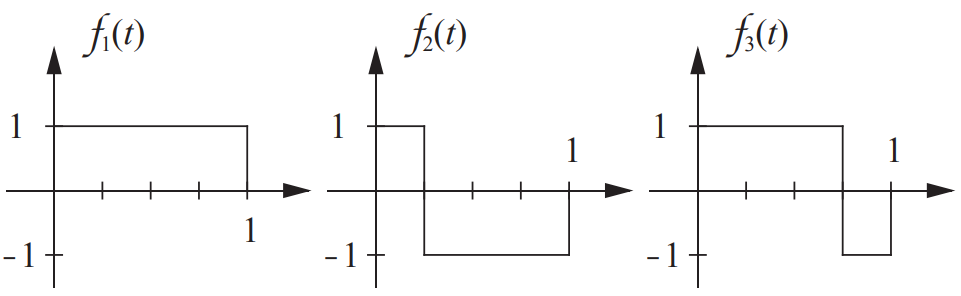
\includegraphics[width=13cm, height=4cm]{151-1}
			
			شکل \lr{E15.1} مجموعه پایه برای تمرین \lr{E5.11}
		\end{center}
	
	
	\hspace{-2.5cm}\textbf{\lr{E5.12}}\hspace{0.6cm}
	فضای بردار تمام توابع پیوسته قطعه را بر روی فاصله \lr{[0,1]} در نظر بگیرید. مجموعه 
	$ \{f_1,f_2\} $
	 ، که در شکل \lr{E15.2} تعریف شده است، شامل دو بردار از این فضای بردار است.
	 \begin{center}
	 	\hspace{-2cm}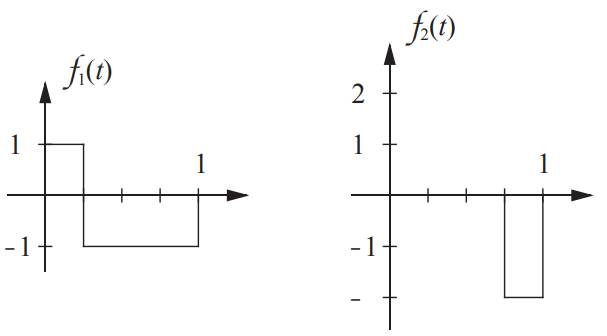
\includegraphics[width=10cm, height=5cm]{151-2}
	 	
	 	شکل \lr{E15.2} مجموعه پایه برای تمرین \lr{E5.12}
	 \end{center}
 
 	\textbf{\lr{.i}}
 با استفاده از روش گرام-اشمیت یک مجموعه متعامد را ایجاد کنید. ضرب داخلی به صورت زیر
 
 \hspace{0.3cm}
  تعریف شده است
	 $$
	 \mathpzc{(f,g)}=\int_{0}^{1}\mathpzc{f(t)g(t)dt}.
	 $$
	 
	 \begin{center}
	 	\hspace{-2cm}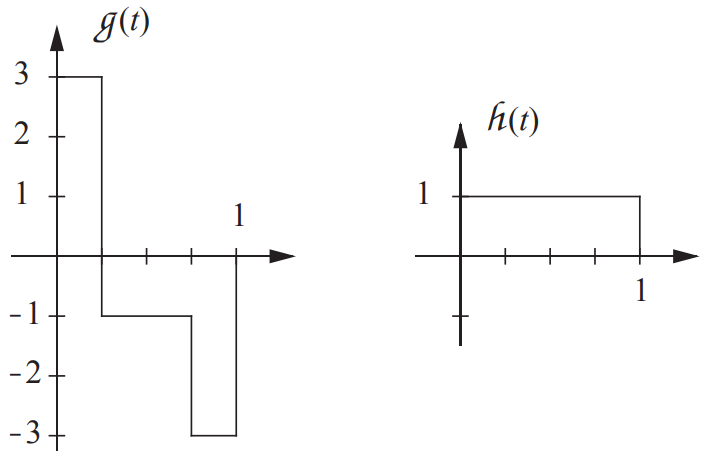
\includegraphics[width=9cm, height=6cm]{152}
	 	
	 شکل \lr{E15.3} بردارهای $ \mathpzc{g} $ و $ \mathpzc{h} $ برای تمرین \lr{E5.12 } قسمت دوم.	 
	 \end{center}
 
 	 \textbf{\lr{.ii}}
 بردارهای $ \mathpzc{g} $ و $ \mathpzc{h} $ را در شکل \lr{E15.3} از نظر مجموعه‌ی متعامدی که در قسمت 1 ایجاد کرده‌اید،
 
 \hspace{0.4cm}
  بسط دهید. در مورد هر مشکلی که پیدا کردید توضیح دهید.\\
 
 \hspace{-2.5cm}\textbf{\lr{E5.13}}\hspace{0.6cm}
مجموعه چند جمله‌ای های درجه 1 یا کمتر را در نظر بگیرید. این یک فضای بردار خطی است. یک پایه برای این فضا به صورت زیر است
	 $$
	 \{\mathpzc{u_1=1,u_2=t}\}
	 $$
	 با استفاده از این مجموعه پایه، چند جمله‌ای $ \mathpzc{y = 2 + 4t} $ را می‌توان به صورت زیر نمایش داد
	 $$
	 \textbf{\lr{y}}_u=
	 \begin{bmatrix}
	 	2 \\ 4
	 \end{bmatrix}
	 $$
	 مجموعه پایه جدید زیر را در نظر بگیرید
	 $$
	 \{\mathpzc{v_1=1+t, v_2=1-t}\}
	 $$
	 برای یافتن نمایشی از $ \mathpzc{y} $ از نظر این مجموعه پایه جدید  از بردارهای پایه متقابل استفاده کنید.\\
	 
	 \hspace{-2.5cm}\textbf{\lr{E5.14}}\hspace{0.6cm}
	 بردار $ \mathpzc{x} $ را می‌توان از نظر بردارهای پایه 
	 $ \{\mathpzc{v_1,v_2}\} $
	  به همان اندازه بسط داد
	  $$
	  \mathpzc{x=1v_1+1v_2}
	  $$
	  بردارهای $ \mathpzc{v1} $ و $ \mathpzc{v2} $ را می‌توان از نظر بردارهای پایه 
	  $ \{\mathpzc{s_1,s_2}\} $
	   به همان اندازه بسط داد
	   $$
	   \mathpzc{v_1=1s_1-1s_2}
	   $$
	   \vspace{-1.2cm}
	   $$
	   \mathpzc{v_2=1s_1+1s_2}
	   $$
	   
	   \textbf{\lr{.i}}
	   از نظر بردارهای پایه $ \mathpzc{\{s_1,s_2\}} $ برای $ \mathpzc{x} $ بسط پیدا کنید.
	   
	   \textbf{\lr{.ii}}
	   بردار $ \mathpzc{y} $ را می‌توان از نظر بردارهای پایه 
	   $ \{\mathpzc{s_1,s_2}\} $
	    گسترش داد
	    $$
	    \mathpzc{y=1s_1+1s_2}
	    $$
	    
	    بسط $ \mathpzc{y} $ را از نظر بردارهای پایه $ \mathpzc{\{s_1,s_2\}} $ پیدا کنید.\\
	    
	    \hspace{-2.5cm}\textbf{\lr{E5.15}}\hspace{0.6cm}
	    فضای بردار تمام توابع پیوسته را روی بازه \lr{[0,1]} در نظر بگیرید. مجموعه $ \mathpzc{\{f_1,f_2\}} $، که در شکل زیر تعریف شده است، شامل دو بردار از این فضای بردار است.
	    \begin{center}
	    	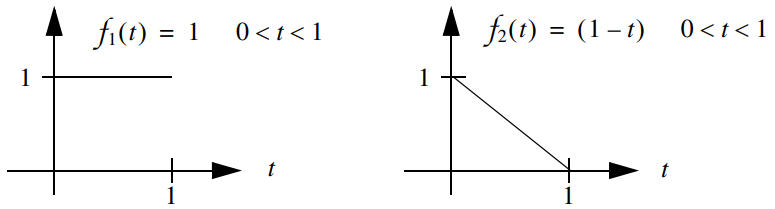
\includegraphics[width=12cm, height=3cm]{153-1}
	    	
	    	شکل \lr{E15.4} بردارهای مستقل برای تمرین \lr{ٍ5.15}
	    \end{center}
    
    \textbf{\lr{.i}}
    با استفاده از روش گرام-اشمیت، از این دو بردار، یک مجموعه متعامد 
    $ \mathpzc{\{g_1,g_2\}} $
     ایجاد کنید.
     
     \hspace{0.3cm}
      ضرب داخلی به صورت زیر تعریف شده است
     $$
     \mathpzc{(f,g)}=\int_{0}^{1}\mathpzc{f(t)g(t)dt}.
     $$
     
     دو بردار متعامد $ \mathpzc{g_1} $ و $ \mathpzc{g_2} $ را به عنوان توابع زمان رسم کنید.\\
     
     \textbf{\lr{.ii}}
     بردار $ \mathpzc{h} $ زیر را از نظر مجموعه ای متعامدی که در قسمت \lr{i} ایجاد کرده‌اید، با استفاده از معادله
     
     \hspace{0.3cm}
      \lr{5.27} بسط دهید. با تولید \lr{h } به عنوان ترکیبی از $ \mathpzc{g_1} $ و $ \mathpzc{g_2} $ نشان دهید که بسط درست است.
     \begin{center}
     	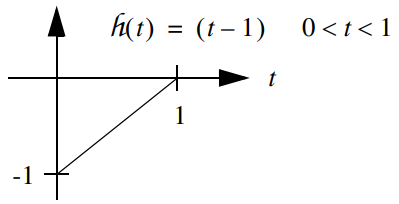
\includegraphics[width=8cm, height=4cm]{153-2}
     	
     	شکل \lr{E15.5} بردار $ \mathpzc{h} $ برای تمرین \lr{E5.15}
     \end{center}
 
 \hspace{-2.5cm}\textbf{\lr{E5.16}}\hspace{0.6cm}
 مجموعه تمام اعداد مختلط را در نظر بگیرید. این را می‌توان یک فضای بردار دانست، زیرا ده ویژگی تعیین کننده را برآورده می‌کند. ما همچنین می‌توانیم یک ضرب داخلی برای این فضای بردار تعیین کنیم
 $ 
 \mathpzc{(x,y)=}Re\mathpzc{(x)}Re\mathpzc{(y)+}Im\mathpzc{(x)}Im\mathpzc{(y)}
 $
، که 
 $ Re\mathpzc{(x)} $
 بخش حقیقی $ \mathpzc{x} $ و 
 $ Im\mathpzc{(x)} $
 بخش موهومی $ \mathpzc{x} $ است.
 
 این منجر به تعریف روبرو برای نُرم می‌شود:
 $ \Vert \mathpzc{x} \Vert = \sqrt{(\mathpzc{x,y})} $.\\
 
 \textbf{\lr{.i}}
 مجموعه پایه زیر را برای فضای بردار توضیح داده شده در بالا در نظر بگیرید: 
 
 \hspace{0.2cm}
 $ \mathpzc{v_1=1+2j, v_2=2+j} $
. بااستفاده ازروش گرام-اشمیت، یک مجموعه پایه متعامد پیداکنید.\\
 
 \textbf{\lr{.ii}}
 با استفاده از مجموعه متعامد خود از قسمت \lr{i.}، بسط‌های برداری را برای 
 
 \hspace{0.4cm}
 $ \mathpzc{u_1=1-j, u_2=1+j} $
 و
 $ \mathpzc{x=3+j} $
  پیدا کنید. این به شما امکان می‌دهد $ \mathpzc{x} $، $ \mathpzc{u_1} $ و 
  
  \hspace{0.4cm}
  $ \mathpzc{u_2} $ را به عنوان ستونی از اعداد
  \textbf{\lr{x}}، $ \textbf{\lr{u}}_1 $
  و
  $ \textbf{\lr{u}}_2 $
   بنویسید.\\
   
   \textbf{\lr{.iii}}
   اکنون می‌خواهیم بردار $ \mathpzc{x} $ را با استفاده از مجموعه پایه    
   $ \{\mathpzc{u_1,u_2}\} $
    نشان دهیم. از بردارهای 
    
    \hspace{0.5cm}
    پایه متقابل استفاده کنید تا بسط را برای $ \mathpzc{x} $ از نظر بردارهای پایه 
    $ \{\mathpzc{u_1,u_2}\} $
     پیدا کنید. این 
     
     \hspace{0.5cm}
     به شما این امکان را می‌دهد که $ \mathpzc{x} $ را به عنوان یک ستون جدید از اعداد 
     $ \textbf{\lr{x}}_u $ 
     بنویسید.\\
     
     \textbf{\lr{.iv}}
     نشان دهید که نمایش‌های $ \mathpzc{x} $ که در قسمت های \lr{ii} و \lr{iii} پیدا کرده اید برابر هستند (دو ستون 
     
     \hspace{0.5cm}
     اعداد $ \textbf{\lr{x}} $ و
      $ \textbf{\lr{x}}^u $
       هر دو یک $ \mathpzc{x} $ را نشان می‌دهند).\\
       
       
        \hspace{-2.5cm}\textbf{\lr{E5.17}}\hspace{0.6cm}
       بردارهای تعریف شده در شکل \lr{E15.6} را در نظر بگیرید. مجموعه 
       $ \{\mathpzc{s_1,s_2}\} $
        مجموعه پایه استاندارد است. مجموعه 
        $ \{\mathpzc{u_1,u_2}\} $
         یک مجموعه پایه جایگزین است. بردار $ \mathpzc{x} $ برداري است كه مي‌خواهيم با توجه به دو مجموعه پايه معرفي كنيم.
         \begin{center}
         	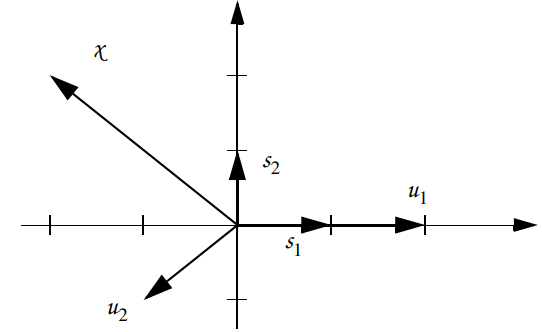
\includegraphics[width=8cm, height=5cm]{154}
         	
         	شکل \lr{E15.6} تعاریف برداری برای تمرین \lr{E15.7}
         \end{center}
     
     \textbf{\lr{.i}}
     از نظر پایه استاندار 
     $ \{\mathpzc{s_1,s_2}\} $
     برای $ \mathpzc{x} $ بسط بنویسید.
     
     \textbf{\lr{.ii}}
     از نظر پایه استاندار 
     $ \{\mathpzc{s_1,s_2}\} $
     برای $ \mathpzc{u_1} $ و $ \mathpzc{u_2} $ بسط بنویسید.
     
     \textbf{\lr{.iii}}
     با استفاده از بردارهای پایه متقابل، از نظر پایه استاندار 
     $ \{\mathpzc{u_1,u_2}\} $
     برای $ \mathpzc{x} $ بسط بنویسید.
     
     \textbf{\lr{.iv}}
     طرح‌هایی رسم کنید،شبیه شکل\lr{5.2}، که نشان می‌دهد بسط قسمت \lr{i} وقسمت \lr{iii} برابرهستند.\\
     
     \hspace{-2.5cm}\textbf{\lr{E5.18}}\hspace{0.6cm}
     مجموعه تمام توابع قابل نوشتن در فرم 
     $ A\sin (t+\theta) $
      را در نظر بگیرید. این مجموعه را می‌توان یک فضای بردار دانست، زیرا ده ویژگی تعریف شده را برآورده می‌کند.\\
            
      \textbf{\lr{.i}}
      مجموعه پایه زیر را برای فضای بردار توضیح داده شده در بالا در نظر بگیرید:
      
      
      $ \mathpzc{v_1=\sin (t), v_2=\cos (t)} $.
      بردار 
      $ \mathpzc{x}=2\sin (t) +4\cos (t) $
       را به عنوان ستونی از اعداد 
       
       \hspace{0.2cm}
       $ \textbf{\lr{x}}^v $
        نشان دهید (با استفاده از این مجموعه پایه، بسط بردار را پیدا کنید).\\
        
        \textbf{\lr{.ii}}
        با استفاده از مجموعه پایه خود از قسمت \lr{i}، بسط‌های برداری را برای 
                        
        $ \mathpzc{u_1}=2\sin (t)+\cos (t), 
        \mathpzc{u_2}=3\sin (t) $
         پیدا کنید.\\
         
         \textbf{\lr{.iii}}
         اکنون می‌خواهیم بردار $ \mathpzc{x} $ قسمت \lr{i} را با استفاده از مجموعه مبنای 
         $ \{\mathpzc{u_1,u_2}\} $
          نشان دهیم. از 
          
          \hspace{0.6cm}
          بردارهای پایه متقابل استفاده کنید تا بسط $ \mathpzc{x} $ را از نظر بردار پایه 
          $ \{\mathpzc{u_1,u_2}\} $
           پیدا کنید. به شما 
           
           \hspace{0.6cm}
           این امکان را می‌دهد که $ \mathpzc{x} $ را به عنوان یک ستون جدید از اعداد 
           $ \textbf{\lr{x}}^u $
            بنویسید.\\
           
           \textbf{\lr{.iv}}
           نشان دهید که نمایش های $ \mathpzc{x} $ که در قسمت های \lr{i} و \lr{iii} پیدا کرده‌اید برابر هستند (دو ستون 
           
           \hspace{0.5cm}
           اعداد 
           $ \textbf{\lr{x}}^v $
            و
           $ \textbf{\lr{x}}^u $
              هر دو یک $ \mathpzc{x} $ یکسان را نشان می‌دهند).\\\\
              
              
        \hspace{-2.5cm}\textbf{\lr{E5.19}}\hspace{0.6cm}  
فرض کنید که ما سه بردار داریم:
$ \mathpzc{x,y,z} \in X $
. می‌خواهیم چند ضرب از $ \mathpzc{y} $ را به $ \mathpzc{x} $ اضافه کنیم، به طوری که بردار حاصل از آن به $ \mathpzc{z} $ متعامد باشد.\\

\textbf{\lr{.i}}
چگونه ضرب مناسب از $ \mathpzc{y} $ را برای اضافه کردن به $ \mathpzc{x} $ تشخیص می‌دهید؟

\textbf{\lr{.ii}}
نتایج خود را با استفاده از بردارهای زیر در قسمت \lr{i} تأیید کنید.
$$
\textbf{\lr{x}}=
\begin{bmatrix}
	1 \\ 0
\end{bmatrix}
\hspace{1cm}
\textbf{\lr{y}}=
\begin{bmatrix}
	1 \\ 0.5
\end{bmatrix}
\hspace{1cm}
\textbf{\lr{z}}=
\begin{bmatrix}
	0.5 \\ 1
\end{bmatrix}
$$

\textbf{\lr{.iii}}
از یک طرح برای نشان دادن نتایج خود از قسمت \lr{ii} استفاده کنید.\\

\hspace{-2.5cm}\textbf{\lr{E5.20}}\hspace{0.6cm}  
$
\textbf{\lr{x}}=
\begin{bmatrix}
	1 & 2 & 2
\end{bmatrix}^T
$
  را از نظر مجموعه پایه زیر بسط دهید. (با استفاده از \lr{MATLAB} پاسخ خود
  
   را تأیید کنید.)
   $$
   \textbf{\lr{v}}_1=
   \begin{bmatrix}
   	-1 \\ 1 \\ 0
   \end{bmatrix}
   \hspace{1cm}
   \textbf{\lr{v}}_2=
   \begin{bmatrix}
   	1 \\ 1 \\ -2
   \end{bmatrix}
   \hspace{1cm}
   \textbf{\lr{v}}_3=
   \begin{bmatrix}
   	1 \\ 1 \\ 0
   \end{bmatrix}
   $$

\hspace{-2.5cm}\textbf{\lr{E5.21}}\hspace{0.6cm}  
مقدار $ a $ را پیدا کنید که 
$ \Vert \mathpzc{x}-a\mathpzc{y} \Vert$
 را حداقل کند. (از 
 $ \Vert \mathpzc{x} \Vert = (\mathpzc{x,x})^{1/2}$
  استفاده کنید.) نشان دهید که برای این مقدار بردار 
  $ \mathpzc{z=x-}a\mathpzc{y} $
   نسبت به $ \mathpzc{y} $ متعامد است و اینکه
   $$
   \Vert \mathpzc{x-}a\mathpzc{y} \Vert^2+
   \Vert a\mathpzc{y} \Vert^2=
   \Vert \mathpzc{x} \Vert^2.
   $$
(بردار 
$ a\mathpzc{y} $
 تصویر $ \mathpzc{x} $ روی $ \mathpzc{y} $ است.) برای حالتی که $ \mathpzc{x} $ و $ \mathpzc{y} $ دو بعدی هستند، نمودار رسم کنید. چگونگی ارتباط این مفهوم با تعامد گرام-اشمیت را توضیح دهید.
\end{document}
